\documentclass[12pt]{article}
\usepackage[utf8]{inputenc}
\usepackage[spanish]{babel}
\usepackage{siunitx}
% ---------------------------------------------------
% 						FONT 
% ---------------------------------------------------

\usepackage{cmbright}								% Font
\documentclass{article}
\usepackage{siunitx}
\usepackage{hyperref} % LINKS
\usepackage{caption}
\decimalpoint
\usepackage{mathtools}
\usepackage{amsmath}
\usepackage{amsthm}
\usepackage{amssymb}
\usepackage{graphicx}
\usepackage[margin=0.9in]{geometry}
\usepackage{fancyhdr}
\usepackage[inline]{enumitem}
\usepackage{float}
\usepackage{cancel}
\usepackage{bigints}
\usepackage{color}
\usepackage{xcolor}
\usepackage{listingsutf8}
\usepackage{algorithm}
\usepackage{tocloft}
\usepackage[none]{hyphenat}
\usepackage{graphicx}
\usepackage{grffile}
\usepackage{tabularx}
\usepackage[nottoc,notlot,notlof]{tocbibind}
\usepackage{times}
\usepackage{color}
\usepackage{enumitem}
\usepackage{amsfonts}
\definecolor{gray97}{gray}{.97}
\definecolor{gray75}{gray}{.75}
\definecolor{gray45}{gray}{.45}
\renewcommand{\cftsecleader}{\cftdotfill{\cftdotsep}}
\pagestyle{fancy}
\setlength{\headheight}{15pt} 
\lhead{Práctica 4: Convertidor Analógico - Digital}
\rhead{\thepage}
\lfoot{ESCOM-IPN}
\renewcommand{\footrulewidth}{0.5pt}
\setlength{\parskip}{0.5em}
\newcommand{\ve}[1]{\overrightarrow{#1}}
\newcommand{\abs}[1]{\left\lvert #1 \right\lvert}
\date{ 01 de Junio 2018}
\title{Amplificador}
\author{Instrumentacion}
\usepackage[
  separate-uncertainty = true,
  multi-part-units = repeat
]{siunitx}

\definecolor{pblue}{rgb}{0.13,0.13,1}
\definecolor{pgreen}{rgb}{0,0.5,0}
\definecolor{pred}{rgb}{0.9,0,0}
\definecolor{pgrey}{rgb}{0.46,0.45,0.48}
\lstset{tabsize=1}
\usepackage{wrapfig}
\usepackage{multicol}
\usepackage{listings}
\lstset{ frame=Ltb,
framerule=0pt,
aboveskip=0.5cm,
framextopmargin=3pt,
framexbottommargin=3pt,
framexleftmargin=0.4cm,
framesep=0pt,
rulesep=.4pt,
backgroundcolor=\color{gray97},
rulesepcolor=\color{black},
%
stringstyle=\ttfamily,
showstringspaces = false,
basicstyle=\small\ttfamily,
commentstyle=\color{gray45},
keywordstyle=\bfseries,
%
numbers=left,
numbersep=15pt,
numberstyle=\tiny,
numberfirstline = false,
breaklines=true,
}

% minimizar fragmentado de listados
\lstnewenvironment{listing}[1][]
{\lstset{#1}\pagebreak[0]}{\pagebreak[0]}

\lstdefinestyle{consola}
{basicstyle=\scriptsize\bf\ttfamily,
backgroundcolor=\color{gray75},
}

\lstdefinestyle{Java}
{language=Java,
}

%%%%%%%%%%%%%%%%%%%%%

\lstdefinestyle{customc}{
  belowcaptionskip=1\baselineskip,
  breaklines=true,
  frame=L,
  xleftmargin=\parindent,
  language=C,
  showstringspaces=false,
  basicstyle=\footnotesize\ttfamily,
  keywordstyle=\bfseries\color{green!40!black},
  commentstyle=\itshape\color{purple!40!black},
  identifierstyle=\color{blue},
  stringstyle=\color{orange},
}

\lstdefinestyle{customasm}{
  belowcaptionskip=1\baselineskip,
  frame=L,
  xleftmargin=\parindent,
  language=[x86masm]Assembler,
  basicstyle=\footnotesize\ttfamily,
  commentstyle=\itshape\color{purple!40!black},
}

\lstset{escapechar=@,style=customc}

% Ayuda para el formato de las tablas
\usepackage{array}
% Se declara un nuevo tipo de columna para alinear de manera:
% -Horizontal
\newcolumntype{P}[1]{>{\centering\arraybackslash}p{#1}}
% -Vertical
\newcolumntype{M}[1]{>{\centering\arraybackslash}m{#1}}

% Indica la separacion entre las columnas de una tabla
\setlength{\tabcolsep}{10pt} % Default value: 6pt
% Indica el padding inferior y superior de las celdas de una tabla
\renewcommand{\arraystretch}{1.8} % Default value: 1

\usepackage{longtable}
%Permite crear columnas en el documento
\usepackage{multicol} 
\usepackage{color}
\usepackage{comment}
\newcommand{\tabitem}{~~\llap{\textbullet}~~}
\newcommand{\subtabitem}{~~~~\llap{\textbullet}~~}

\bibliographystyle{IEEEtran}
\begin{document}
		\begin{titlepage}
			\begin{center}
				
				% Upper part of the page. The '~' is needed because \\
				% only works if a paragraph has started.
				
				\noindent
				\begin{minipage}{0.5\textwidth}
					\begin{flushleft} \large
						\includegraphics[width=0.5\textwidth]{../ipn.png}
					\end{flushleft}
				\end{minipage}%
				\begin{minipage}{0.55\textwidth}
					\begin{flushright} \large
						\includegraphics[width=0.4\textwidth]{../escom.png}
					\end{flushright}
				\end{minipage}
				
				\textsc{\LARGE Instituto Politécnico Nacional}\\[0.5cm]
				
				\textsc{\Large Escuela Superior de Cómputo}\\[1cm]
				
				% Title
				
				{ \huge Práctica 4: Convertidor Analógico - Digital \\[1cm] }
				
				{ \Large Unidad de aprendizaje: Instrumentación} \\[1cm]
				
				{ \Large Grupo: 3CM4 } \\[1cm]
				
				\noindent
				\begin{minipage}{0.5\textwidth}
					\begin{flushleft} \large
						\emph{Integrantes:}\\
						
						\begin{tabular}{ll}
						Aguilar Herrera Arianna Itzamina \\
					    Nicolás Sayago Abigail\\
					    Ramos Diaz Enrique \\
					\end{tabular}
					\end{flushleft}
				\end{minipage}%
				\begin{minipage}{0.5\textwidth}
					\begin{flushright} \large
						\emph{Profesor(a):} \\
						Tellez Barrera Juan Carlos  \\
					\end{flushright}
				\end{minipage}
				
				\vfill
				
				% Bottom of the page
				{\large Fecha de entrega: 19 de octubre de 2018}
			\end{center}
		\end{titlepage}
	
	\tableofcontents
	\newpage
	
	% /////////////////////////////////////////////////////////////////////
	%							OBJETIVOS
	% ////////////////////////////////////////////////////////////////////
	\section{Objetivo}
	\begin{itemize}
	    \item[\checkmark] Estudiar las características del convertidor Analógico – Digital (A/D) ADC0809.
        \item[\checkmark] Aplicar los conceptos de resolución y determinación de error.
        \item[\checkmark] Utilizar el ADC0809 para realizar una aplicación de sensado de temperatura
	\end{itemize}
	
	% /////////////////////////////////////////////////////////////////////
	%							MATERIAL
	% ////////////////////////////////////////////////////////////////////

	\section{Material de referencia}
	\begin{itemize}
	    \item Apuntes de Clase
\item Investigación en Internet
\item Hojas de Datos del ADC0809.
	\end{itemize}
	
		% /////////////////////////////////////////////////////////////////////
	%							EQUIPO
	% ////////////////////////////////////////////////////////////////////
		\section{Listado de materiales}
		
		\begin{multicols}{2}
	
	\begin{itemize}
	    \item 1 Convertidor Analógico Digital ADC0809
        \item 9 Resistores $2.7 K\Omega$
        \item 11 Leds
        \item 1	Circuito Integrado 74HC14
        \item 1	Capacitor 1.5 nF
        \item 1	Resistor de $2.2 K\Omega$ 
        \item 1	Diodo IN4001 a 7
        \end{itemize}

	  
	  \columnbreak
	  
	  \begin{itemize}
	      \item 1 Amplificador Operacional LM741
	      \item 11 Resistores de $1 K\Omega$
        \item 1 Circuito integrado LM35
        \item 1 Dipswitch de 3 entradas
        \item 2	Resistores según cálculos
        \item 1	Regulador 7805

	  \end{itemize}
	  
	  \end{multicols}
	  
	  \section{Listado de equipo}
	\begin{itemize}
	    \item 1	Voltímetro digital.
        \item 1	Fuente de alimentación.
        \item 1	Osciloscopio digital

	    \end{itemize}
	    
	
	% /////////////////////////////////////////////////////////////////////
	%							INTRODUCCION
	% ////////////////////////////////////////////////////////////////////

	\section{Introducción}
	\subsection{Convertidor ADC0809}
	Para nuestra práctica utilizaremos el   convertidor \textbf{ADC0809}. Este es un conversor de 8 bits (la señal análoga se convierte en una palabra digital de 8 bits), que tiene la posibilidad de leer 8 señales analógicas (8 canales). Posee 28 pines de los cuales 8 corresponden a sus canales analógicos de entrada; éste solo puede leer un canal a la vez y dispone por lo tanto de un selector (multiplexor) de 3 líneas,  que permite seleccionar la señal de entrada a convertir, mediante el código binario presente en estas entradas de selección. Posee un tiempo de conversión de 100 microsegundos y una entrada máxima de reloj de 500 KHz.
	
	\begin{figure}[h!]
                \centering
                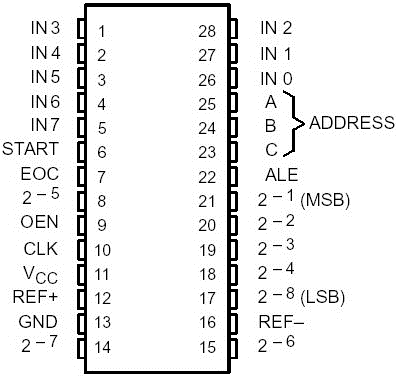
\includegraphics[scale=0.75]{Practica4/Images/adc.png}
                \caption{Circuito integrado ADC0809}
    \end{figure} 
	
	\subsection{Descripción de las líneas del ADC0809}

	\item \textbf{Entradas Analógicas (IN0…IN7):} Líneas de entrada de las señales análogas que se quiere digitalizar.

    \item \textbf{Bus de salida de datos ($2^{-8}$…$2^{-1}$):} Estas líneas de salida entregan la palabra binaria que corresponde al nivel análogo de entrada (poseen tri-state).

    \item \textbf{OE (Habilitación de salida):} Con esta línea se habilita la salida. Cuando OE  esta en ‘0’ la salida permanece en tri-state, cuando esta a ‘1’ entrega el código digital de salida.

    \item \textbf{START:} Entrada para indicar al ADC que debe iniciar un nuevo ciclo de conversión.

    \item \textbf{EOC (Fin de conversión):} Cuando el proceso de conversión finaliza, el ADC emite esta señal para indicar que en el bus de datos del mismo hay una palabra digital.

    \item \textbf{CLK (Clock):} Es la entrada correspondiente a la señal de reloj.
    
        
        \subfigure{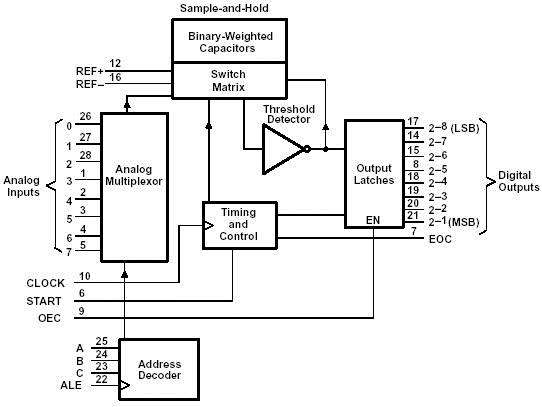
\includegraphics[scale=0.75]{Practica4/Images/img2.png}}
        \subfigure{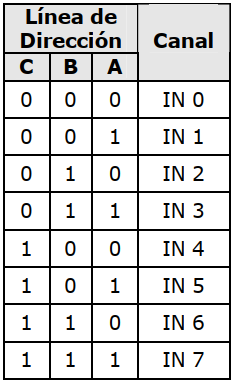
\includegraphics[scale=0.6]{Practica4/Images/img4.PNG}}

    
    \subsection{Funcionamiento}
    El \textbf{ADC0808} usa la técnica de aproximaciones sucesivas para la conversión. Esta técnica es usada en A/D de bajo costo, resolución media y alta velocidad.
    
    El ciclo empieza al aplicar una señal analógica a la entrada y colocar un pulso en \textbf{START}. 
    
    El primer pulso de reloj en el \textbf{S.A.R} (successive approximation register) coloca en 1 la salida del MSB. Este valor hace que el DAC  coloque  en  su  salida  el  50\%	de su valor total. El \textbf{S.A.R} mira  la  salida  del comparador  para saber  si  la  salida  análoga del DAC es mayor o menor que la señal análoga de entrada.
    
    Si el voltaje del \textbf{DAC} es mayor, el comparador coloca su salida en cero. Esto hace que el S.A.R también coloque en ‘0’ su MSB.
    
    Si el voltaje en la salida del DAC es menor que el de la señal de entrada, el comparador coloca en ‘1’ su salida y el S.A.R mantiene en ‘1’ su MSB. Todo lo anterior ha ocurrido en un solo pulso de reloj.
    
    El \textbf{S.A.R} examina todos los bits, desde el MSB al LSB. Ya que un bit se evalúa en cada pulso de reloj, un ADC de 8 bits empleará, en la conversión solamente 8 pulsos de reloj. Cuando se ha procesado el último bit, el S.A.R envía una señal de fin de conversión \textbf{(EOC)}, que permite el almacenamiento de la palabra resultante en el registro de salida. Después de seleccionar el canal (3 bits) y dar la señal de \textbf{START}, el circuito emplea 100uS para completar el proceso; cuando esto ocurre, coloca los ocho bits de la palabra digital resultante en un registro tri-state de almacenamiento en la salida y emite la señal \textbf{EOC}.
    
    Las  referencias  \textbf{REF+}  y \textbf{REF-}  permiten  calibrar  el rango de  conversión.  Conectando
    \textbf{REF+} a 5V y \textbf{REF-} a 0V, la salida será 00h para 0V y FFh para 5V de la señal de entrada.
    
    \subsection{Procedimiento para la lectura del Convertidor}
    \begin{multicols}{2}
			Para iniciar una nueva conversión de la señal de cualquiera de los ocho canales, se realizan los siguientes pasos:
    
    \begin{enumerate}
        \item Colocar el código de selección de canal (\textbf{CBA})
        \item Generar la señal \textbf{ALE} y \textbf{START}.
        \item Esperar que el Conversor emita la señal \textbf{EOC}.
        \item Activar señal \textbf{OE} (para sacar de tri-state las salidas).
        \item Leer el dato digital por la salida del ADC.
        
    \end{enumerate}

	\columnbreak

	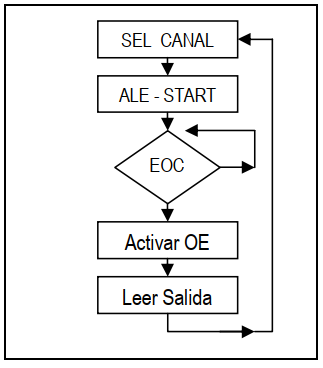
\includegraphics[width=0.4\textwidth]{Practica4/Images/img5.PNG}
    \end{multicols}

    \textbf{Es importante tener en cuenta que para realizar la lectura de los canales del conversor AD adecuadamente se deben además respetar todos los tiempos de las señales necesarias. Para esto se debe recurrir a la hoja de datos del convertidor.}
    
    Observa el siguiente diagrama de tiempos del conversor ADC0809. Es importante interpretar este diagrama ya que en el se puede entender el comportamiento de este dispositivo.
    
    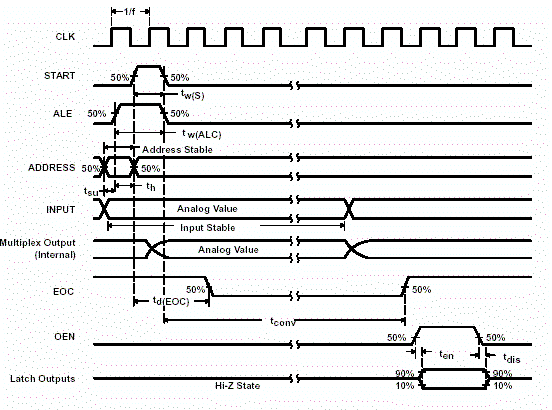
\includegraphics[width=0.85\textwidth]{Practica4/Images/img3.png}
    



	% /////////////////////////////////////////////////////////////////////
	%							DESARROLLO
	% ////////////////////////////////////////////////////////////////////
    \newpage
	\section{Desarrollo práctico}
	\subsection{PE 1 - Características del ADC0809}
	Usando la hoja de datos del ADC0809 completar los siguientes puntos.
    \begin{figure}[h!]
                \centering
                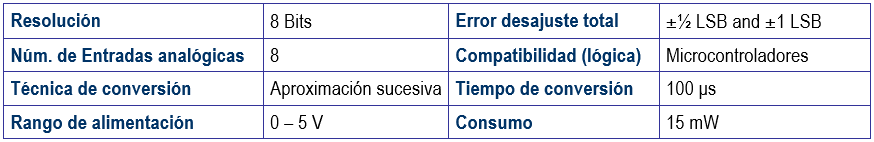
\includegraphics[width=0.95\textwidth]{Practica4/Images/tabla1.PNG}
    \end{figure}
    
	% ---------------------------------------------------------
	\subsection{PE 2 - Funcionamiento del convertidor ADC0809 }
	\subsubsection{Construya el siguiente circuito de prueba}
	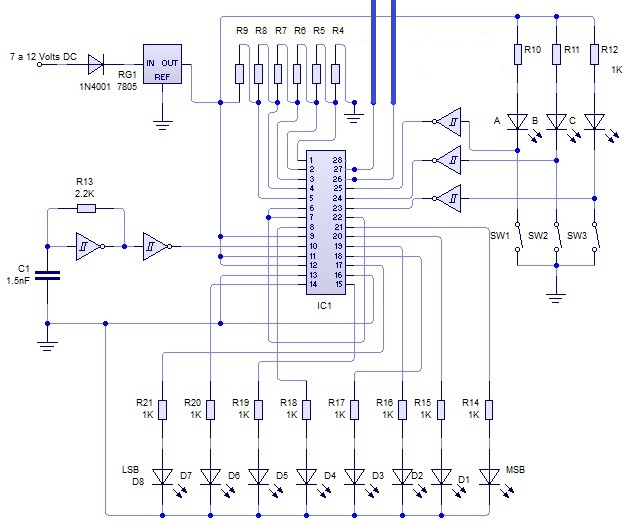
\includegraphics[width=0.95\textwidth]{Practica4/Images/cad.png}
	\subsubsection{Circuito cableado}
	\begin{figure}[h!]
                \centering
                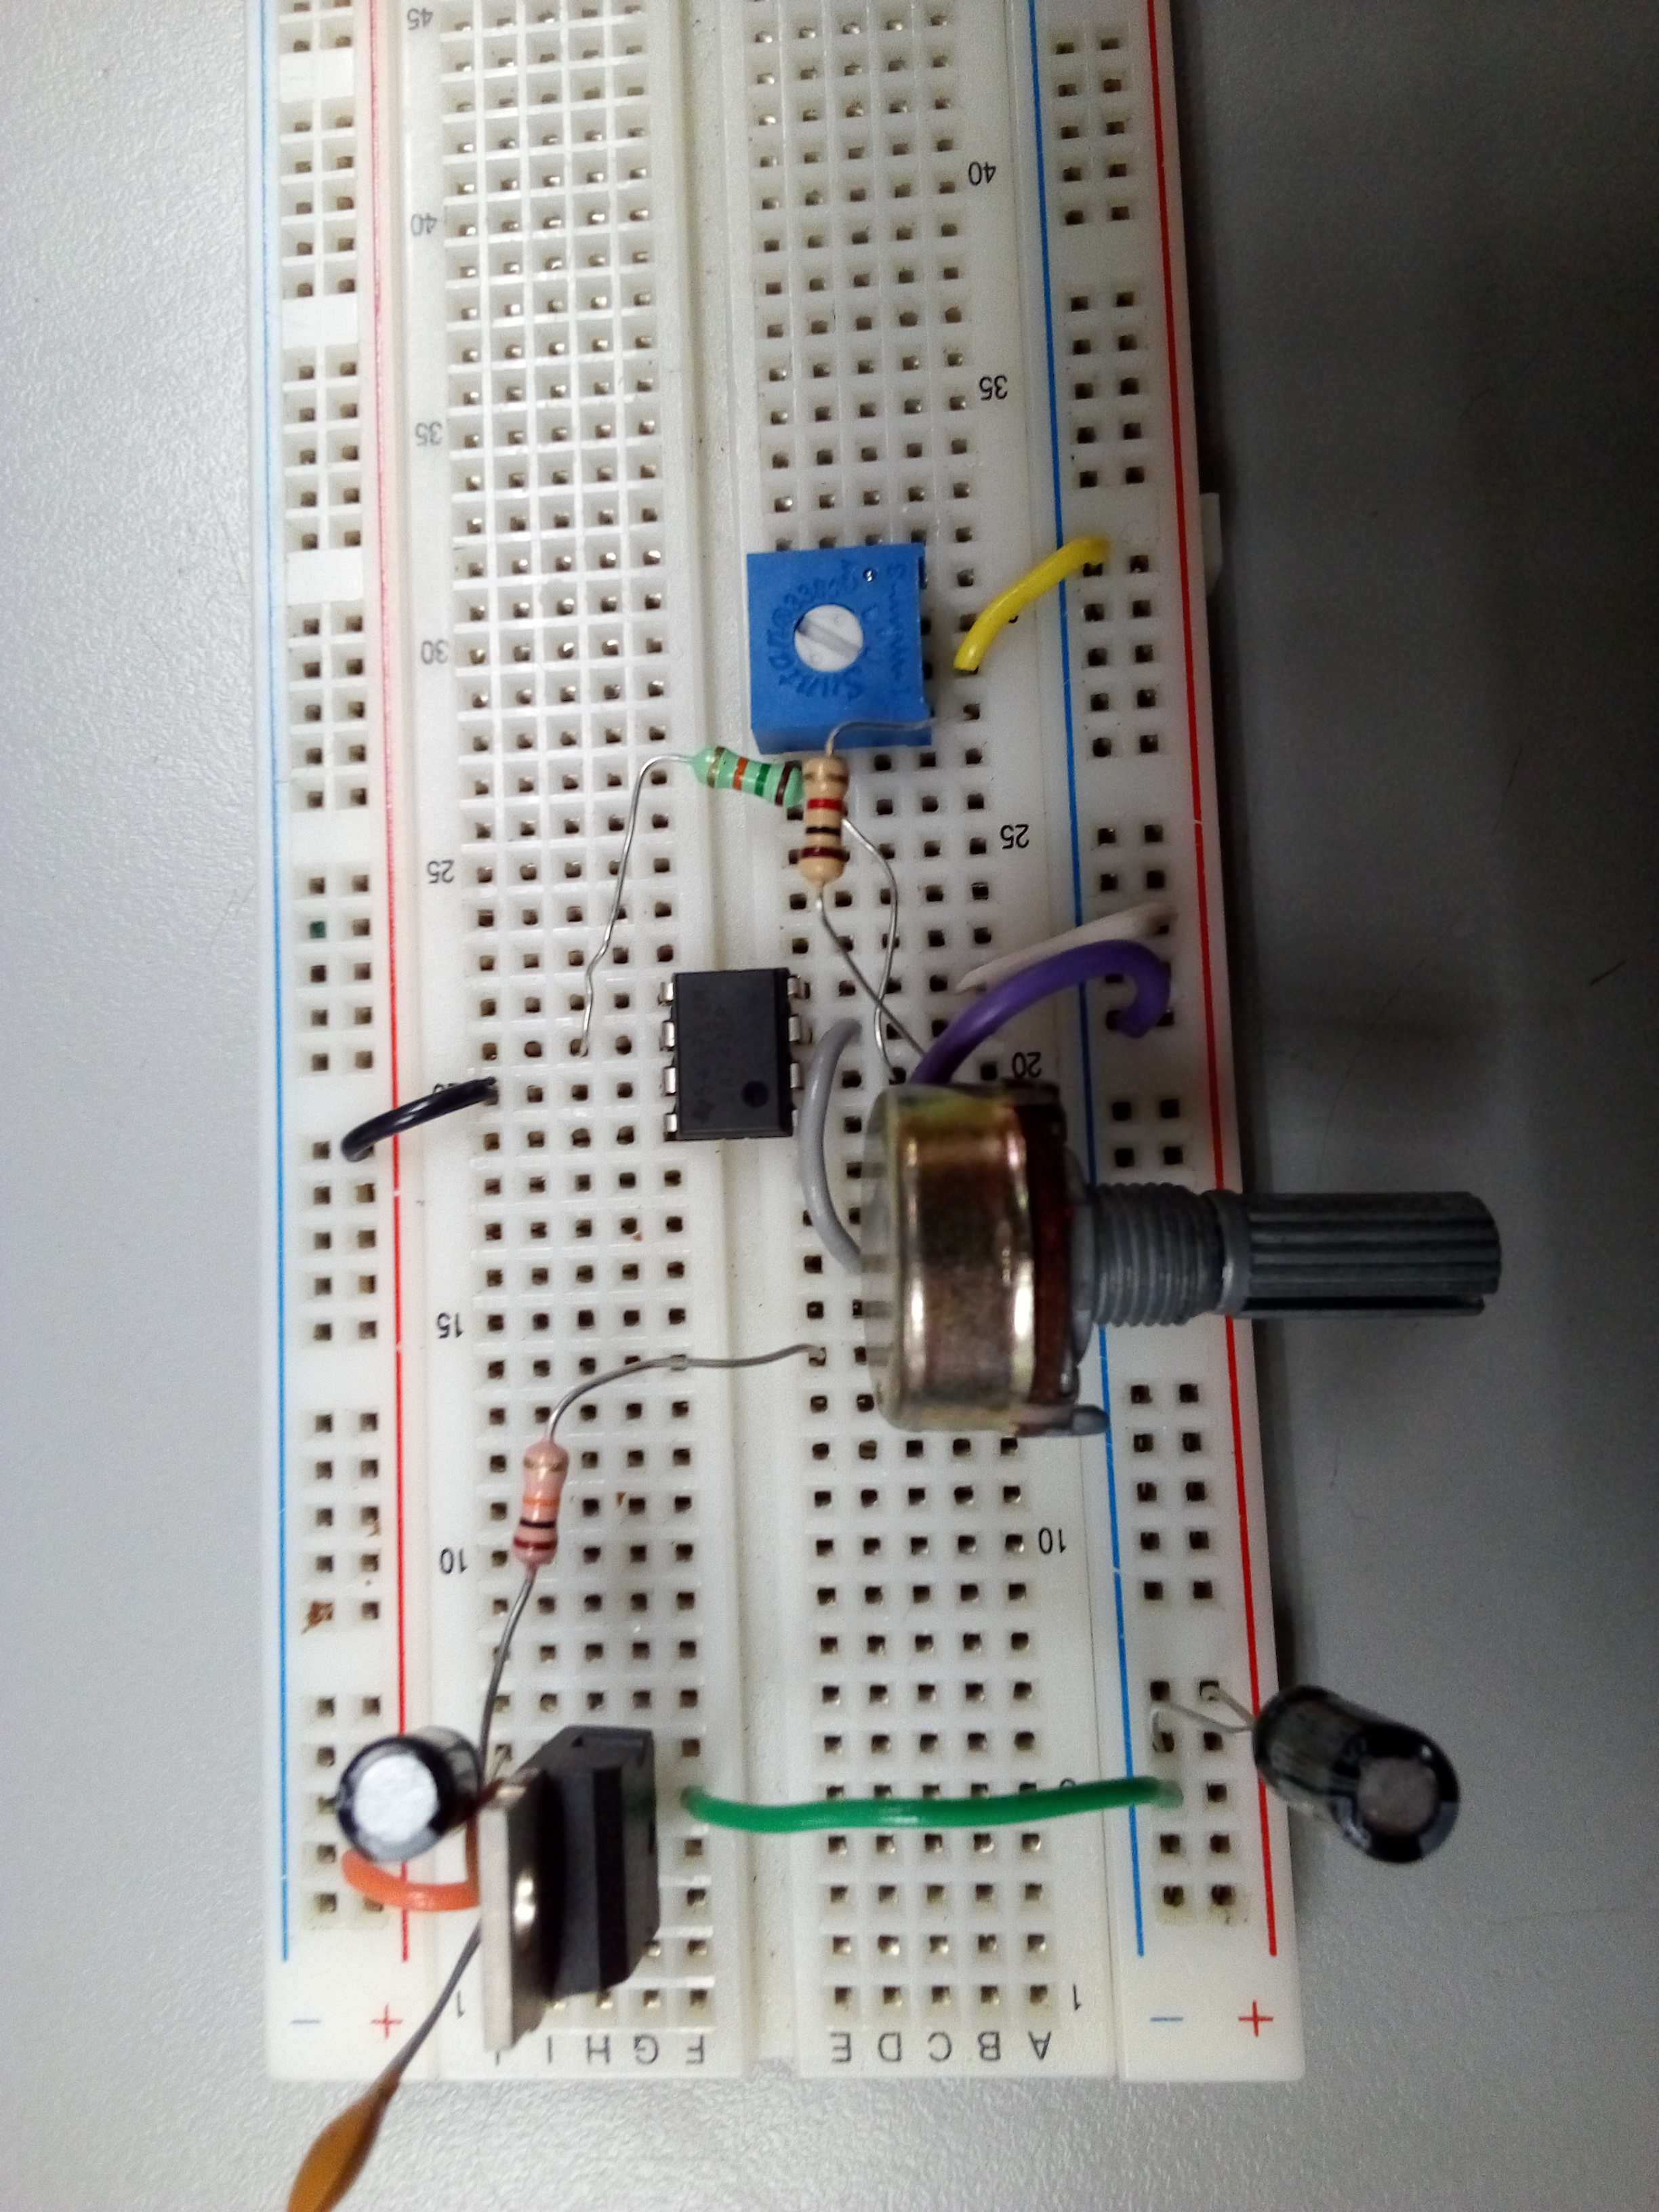
\includegraphics[width=0.9\textwidth]{Practica4/Fotos/circuito2.jpg}
    \end{figure}
	\subsubsection{Procedimiento Experimental}
	En el divisor resistivo, medir el voltaje correspondiente a las entradas análogas de IN0 hasta IN7. 
	
	Calcular la resolución de voltaje en el convertidor tomando en cuenta que es de 8 bits y la entrada de referencia que es de 5 volts. Determinar el valor correspondiente de acuerdo al valor numérico en decimal y en binario, el cual sera comparado con el valor reflejado en las salidas digitales. Determinar el error en cada una de las lecturas correspondientes a cada canal.
	
	\textbf{Resolución = } $\frac{V_{CC}}{8 bits} = \frac{5 V}{255} = 0.019607 V$ 
	
	\newpage
	\subsubsection{Tabla de mediciones}
	\begin{figure}[h!]
                \centering
                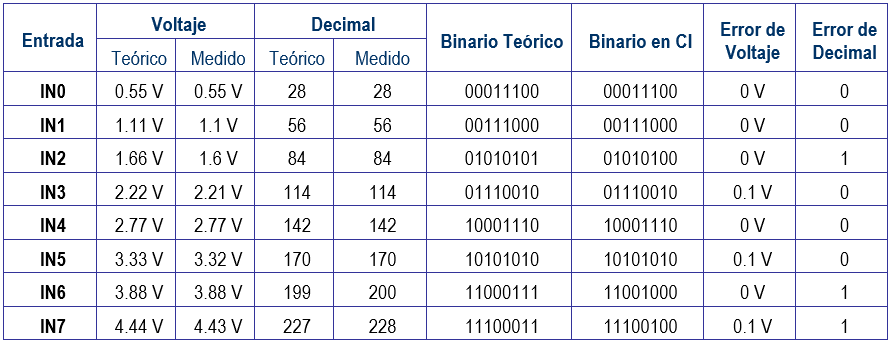
\includegraphics[width=\textwidth]{Practica4/Images/tabla2.PNG}
    \end{figure}
    
    \textbf{Canal 0}
    \begin{figure}[h!]
                \centering
                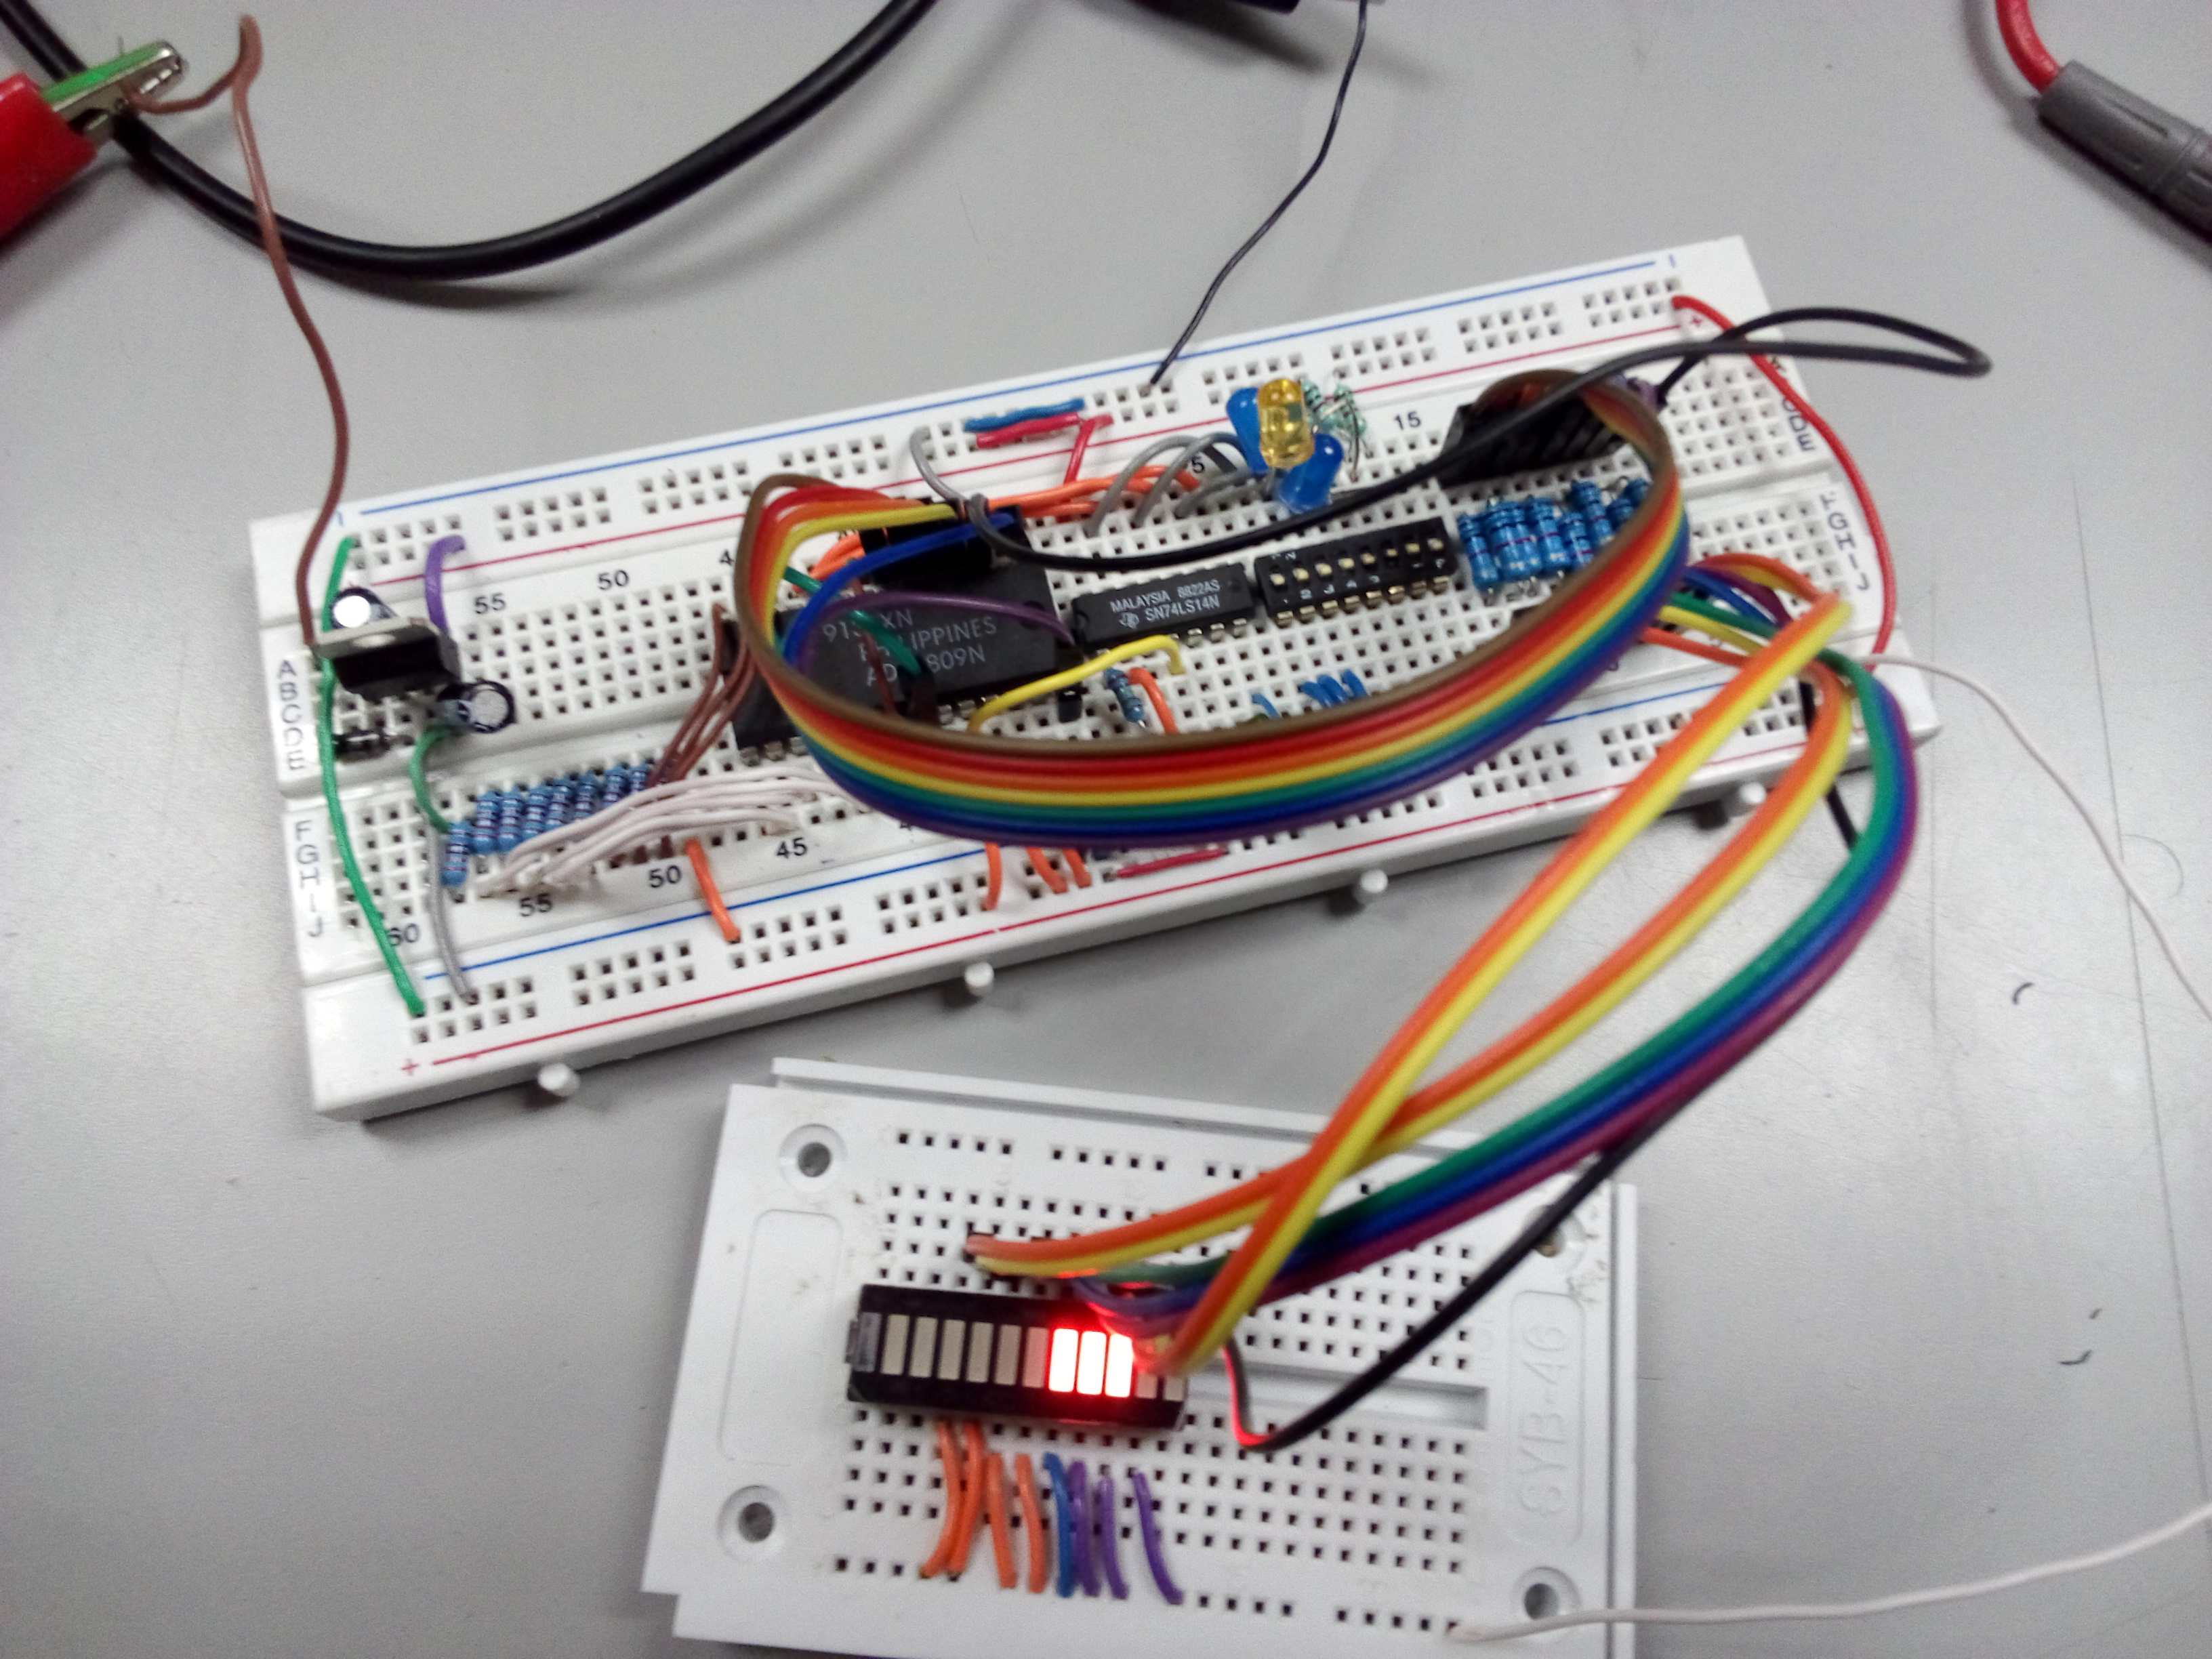
\includegraphics[width=0.71\textwidth]{Practica4/Fotos/canal0.jpg}
    \end{figure}
    \newpage
    \textbf{Canal 1}
    \begin{figure}[h!]
                \centering
                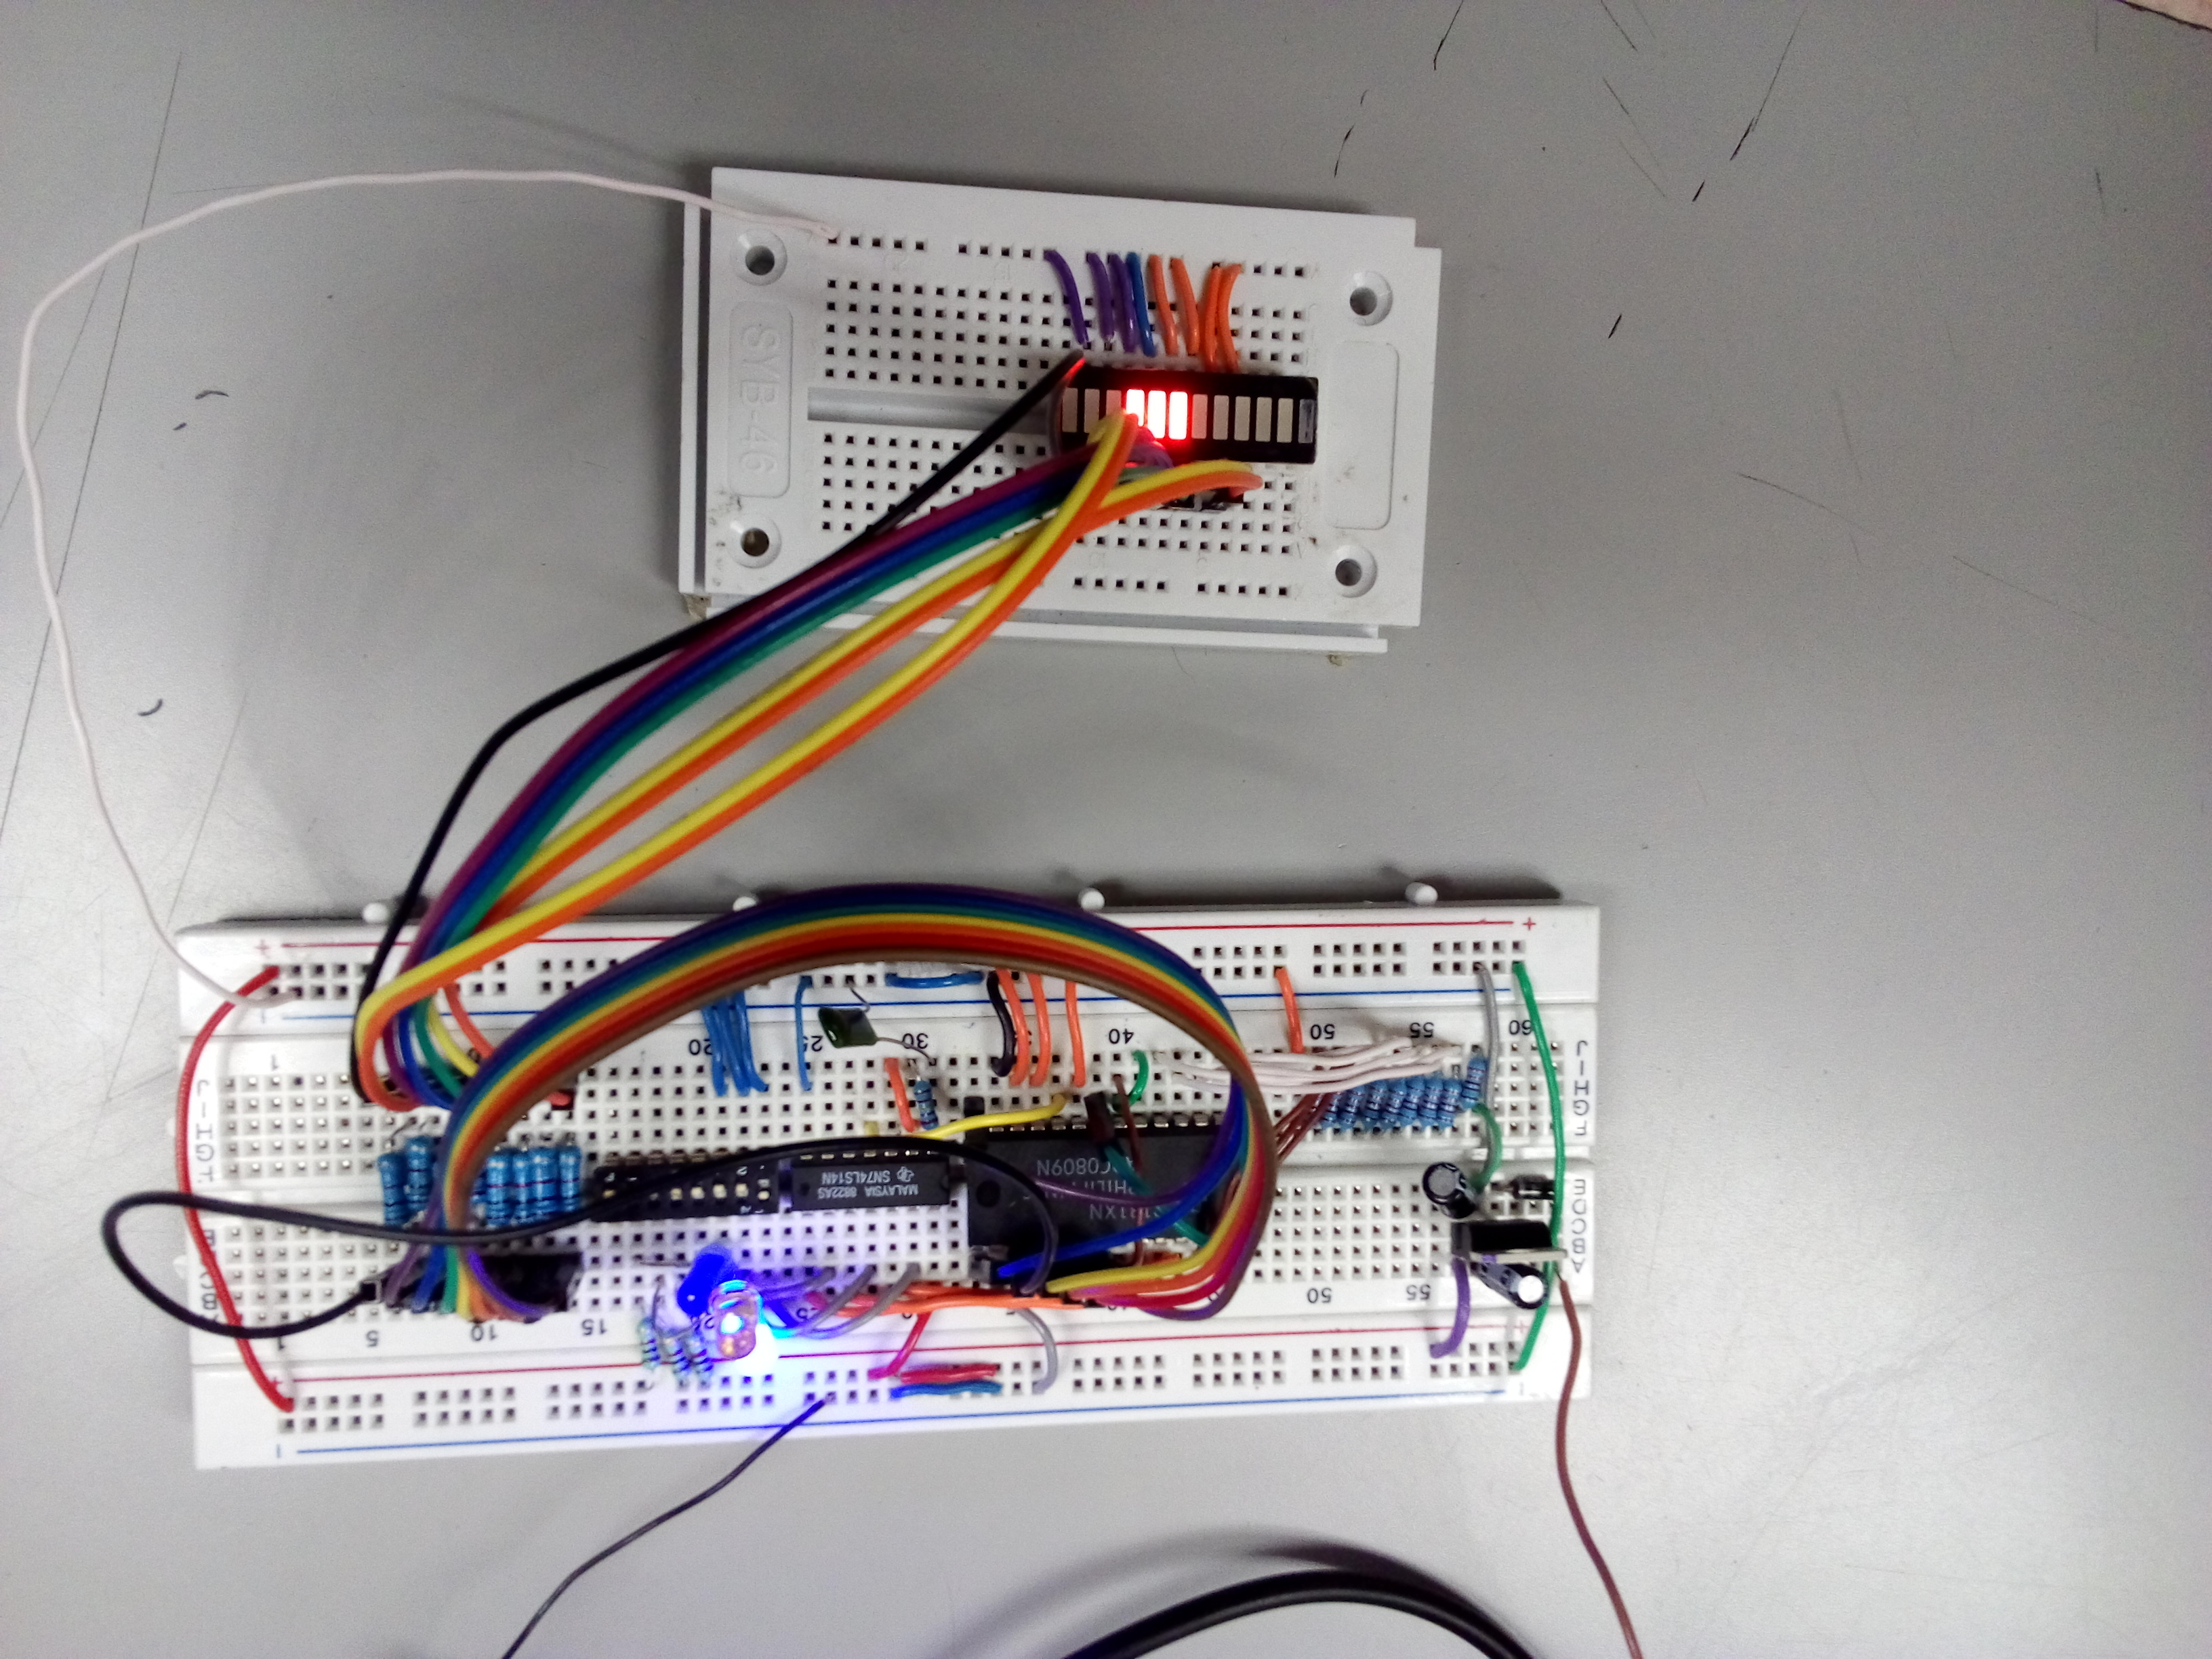
\includegraphics[width=0.71\textwidth]{Practica4/Fotos/canal1.jpg}
    \end{figure}
    
    \textbf{Canal 2}
    \begin{figure}[h!]
                \centering
                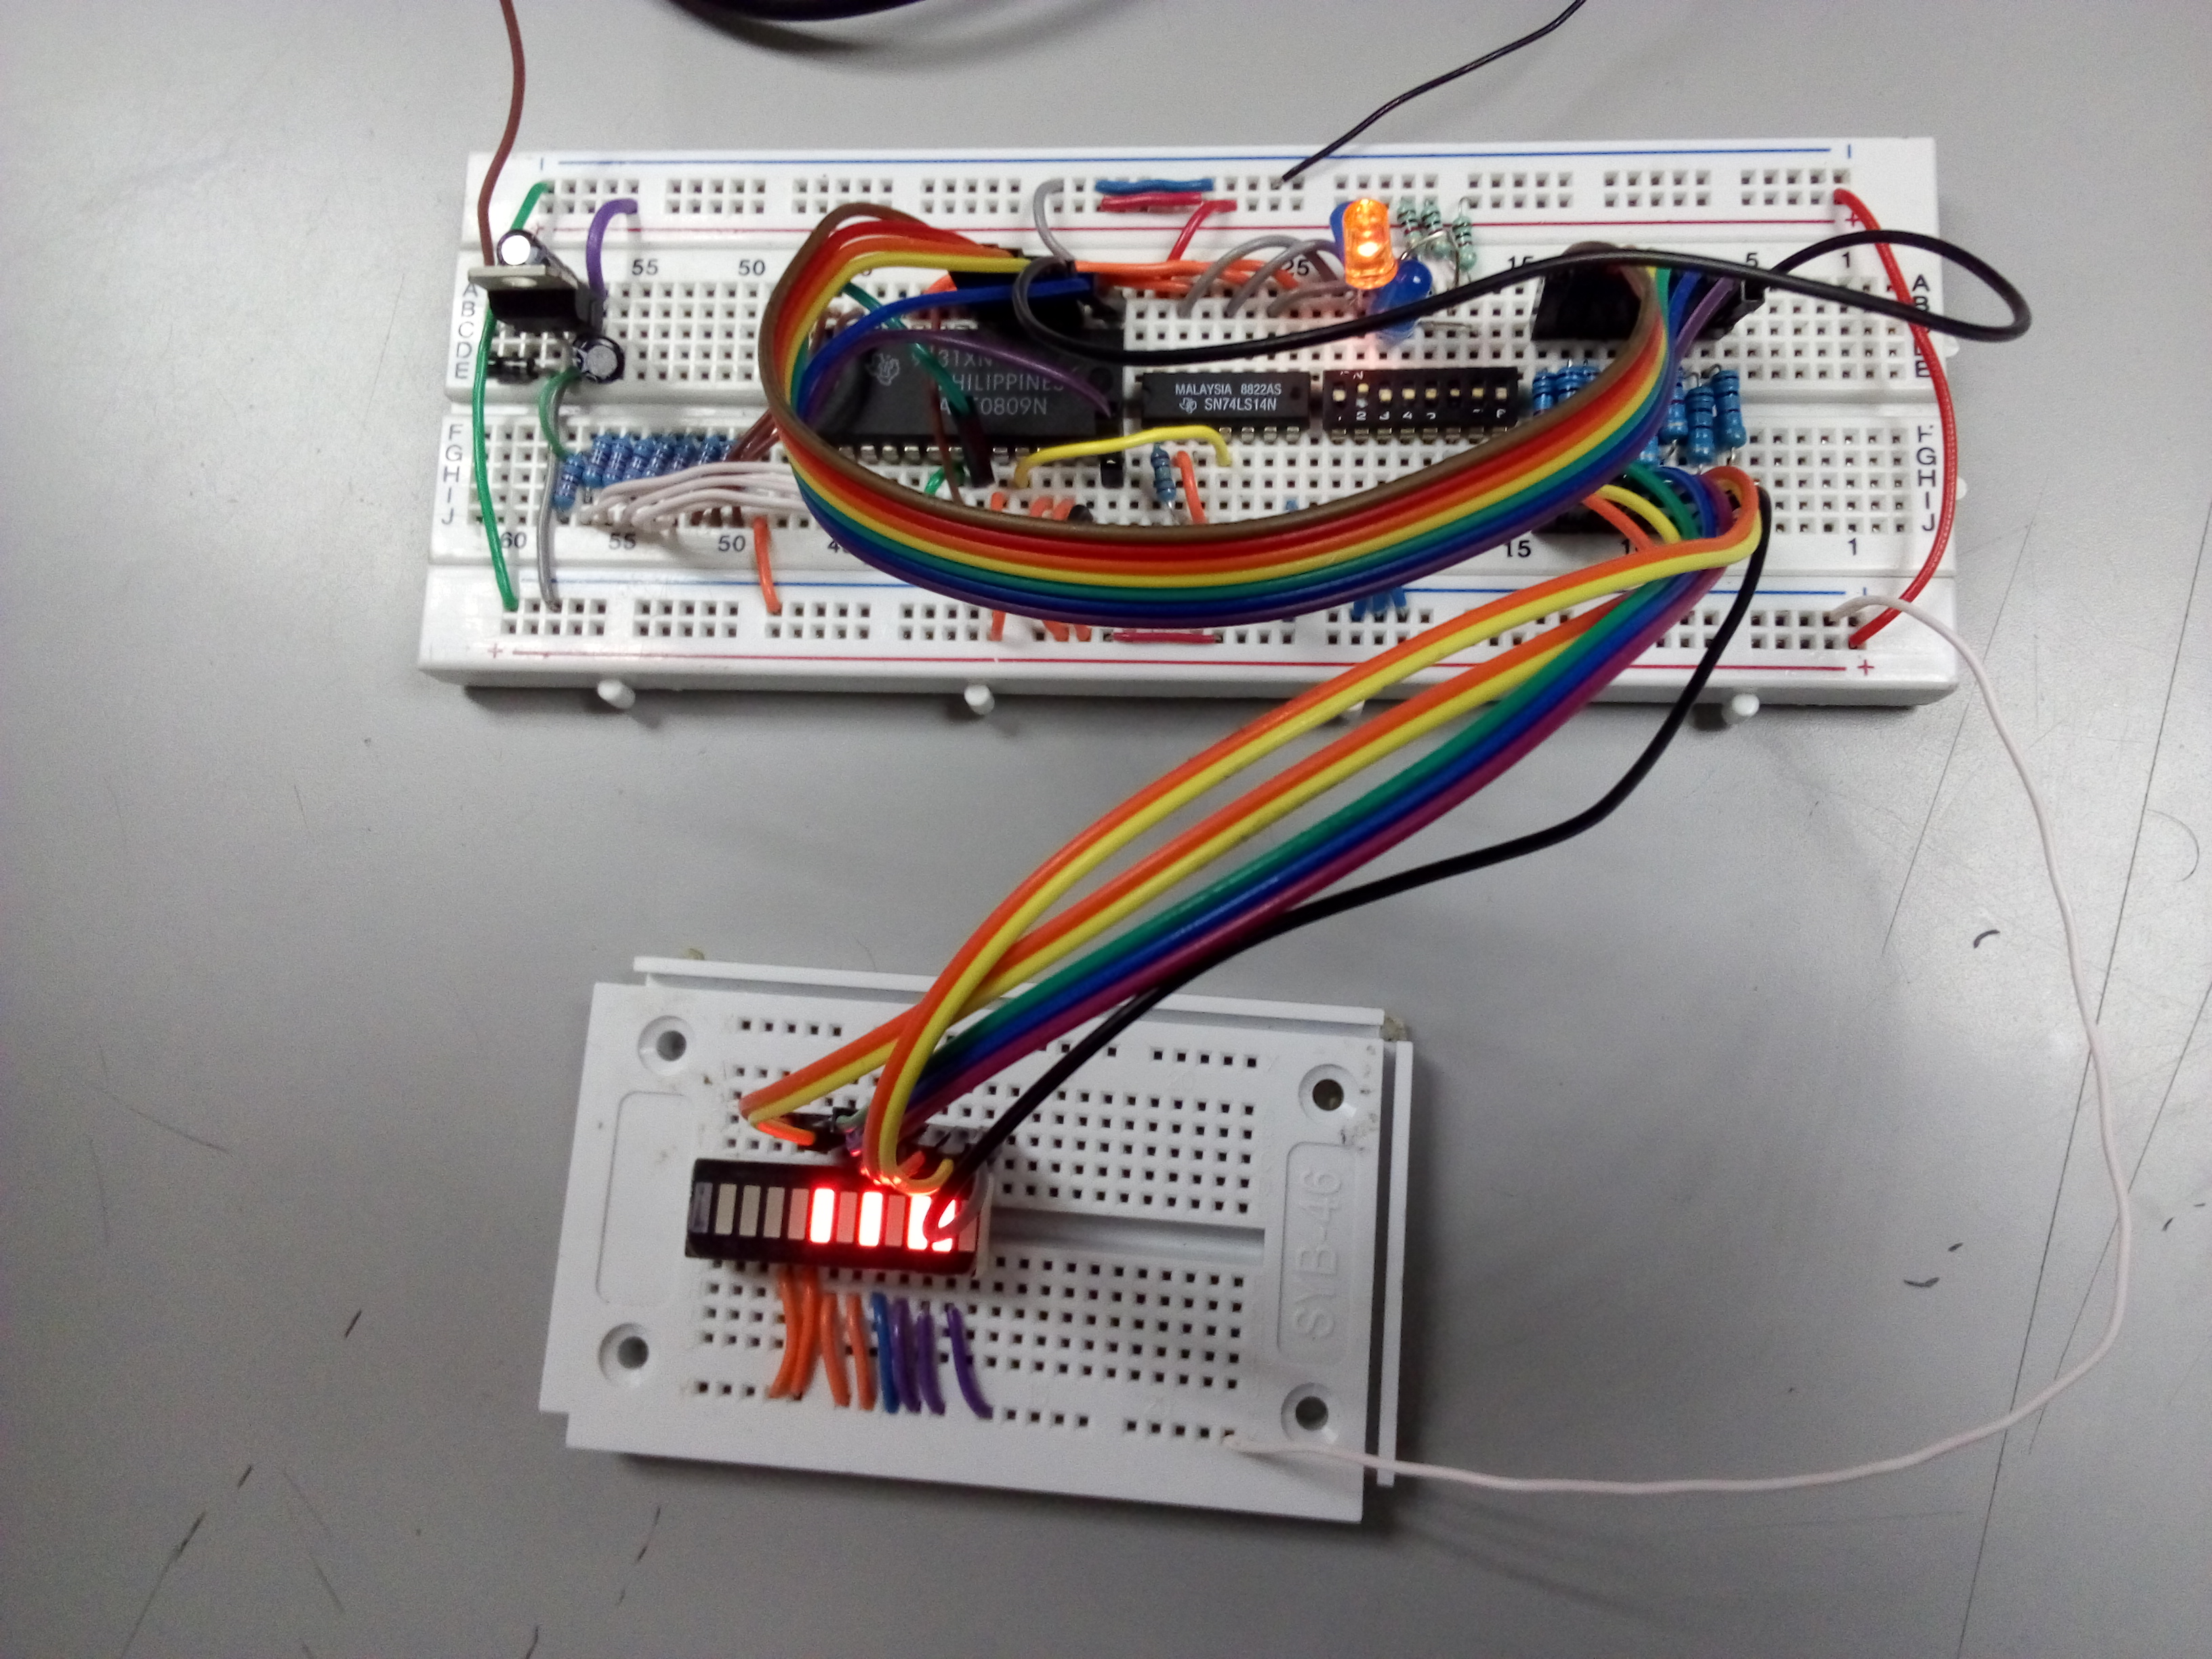
\includegraphics[width=0.71\textwidth]{Practica4/Fotos/canal2_1.jpg}
    \end{figure}
    
    \newpage
    \textbf{Canal 3}
    \begin{figure}[h!]
                \centering
                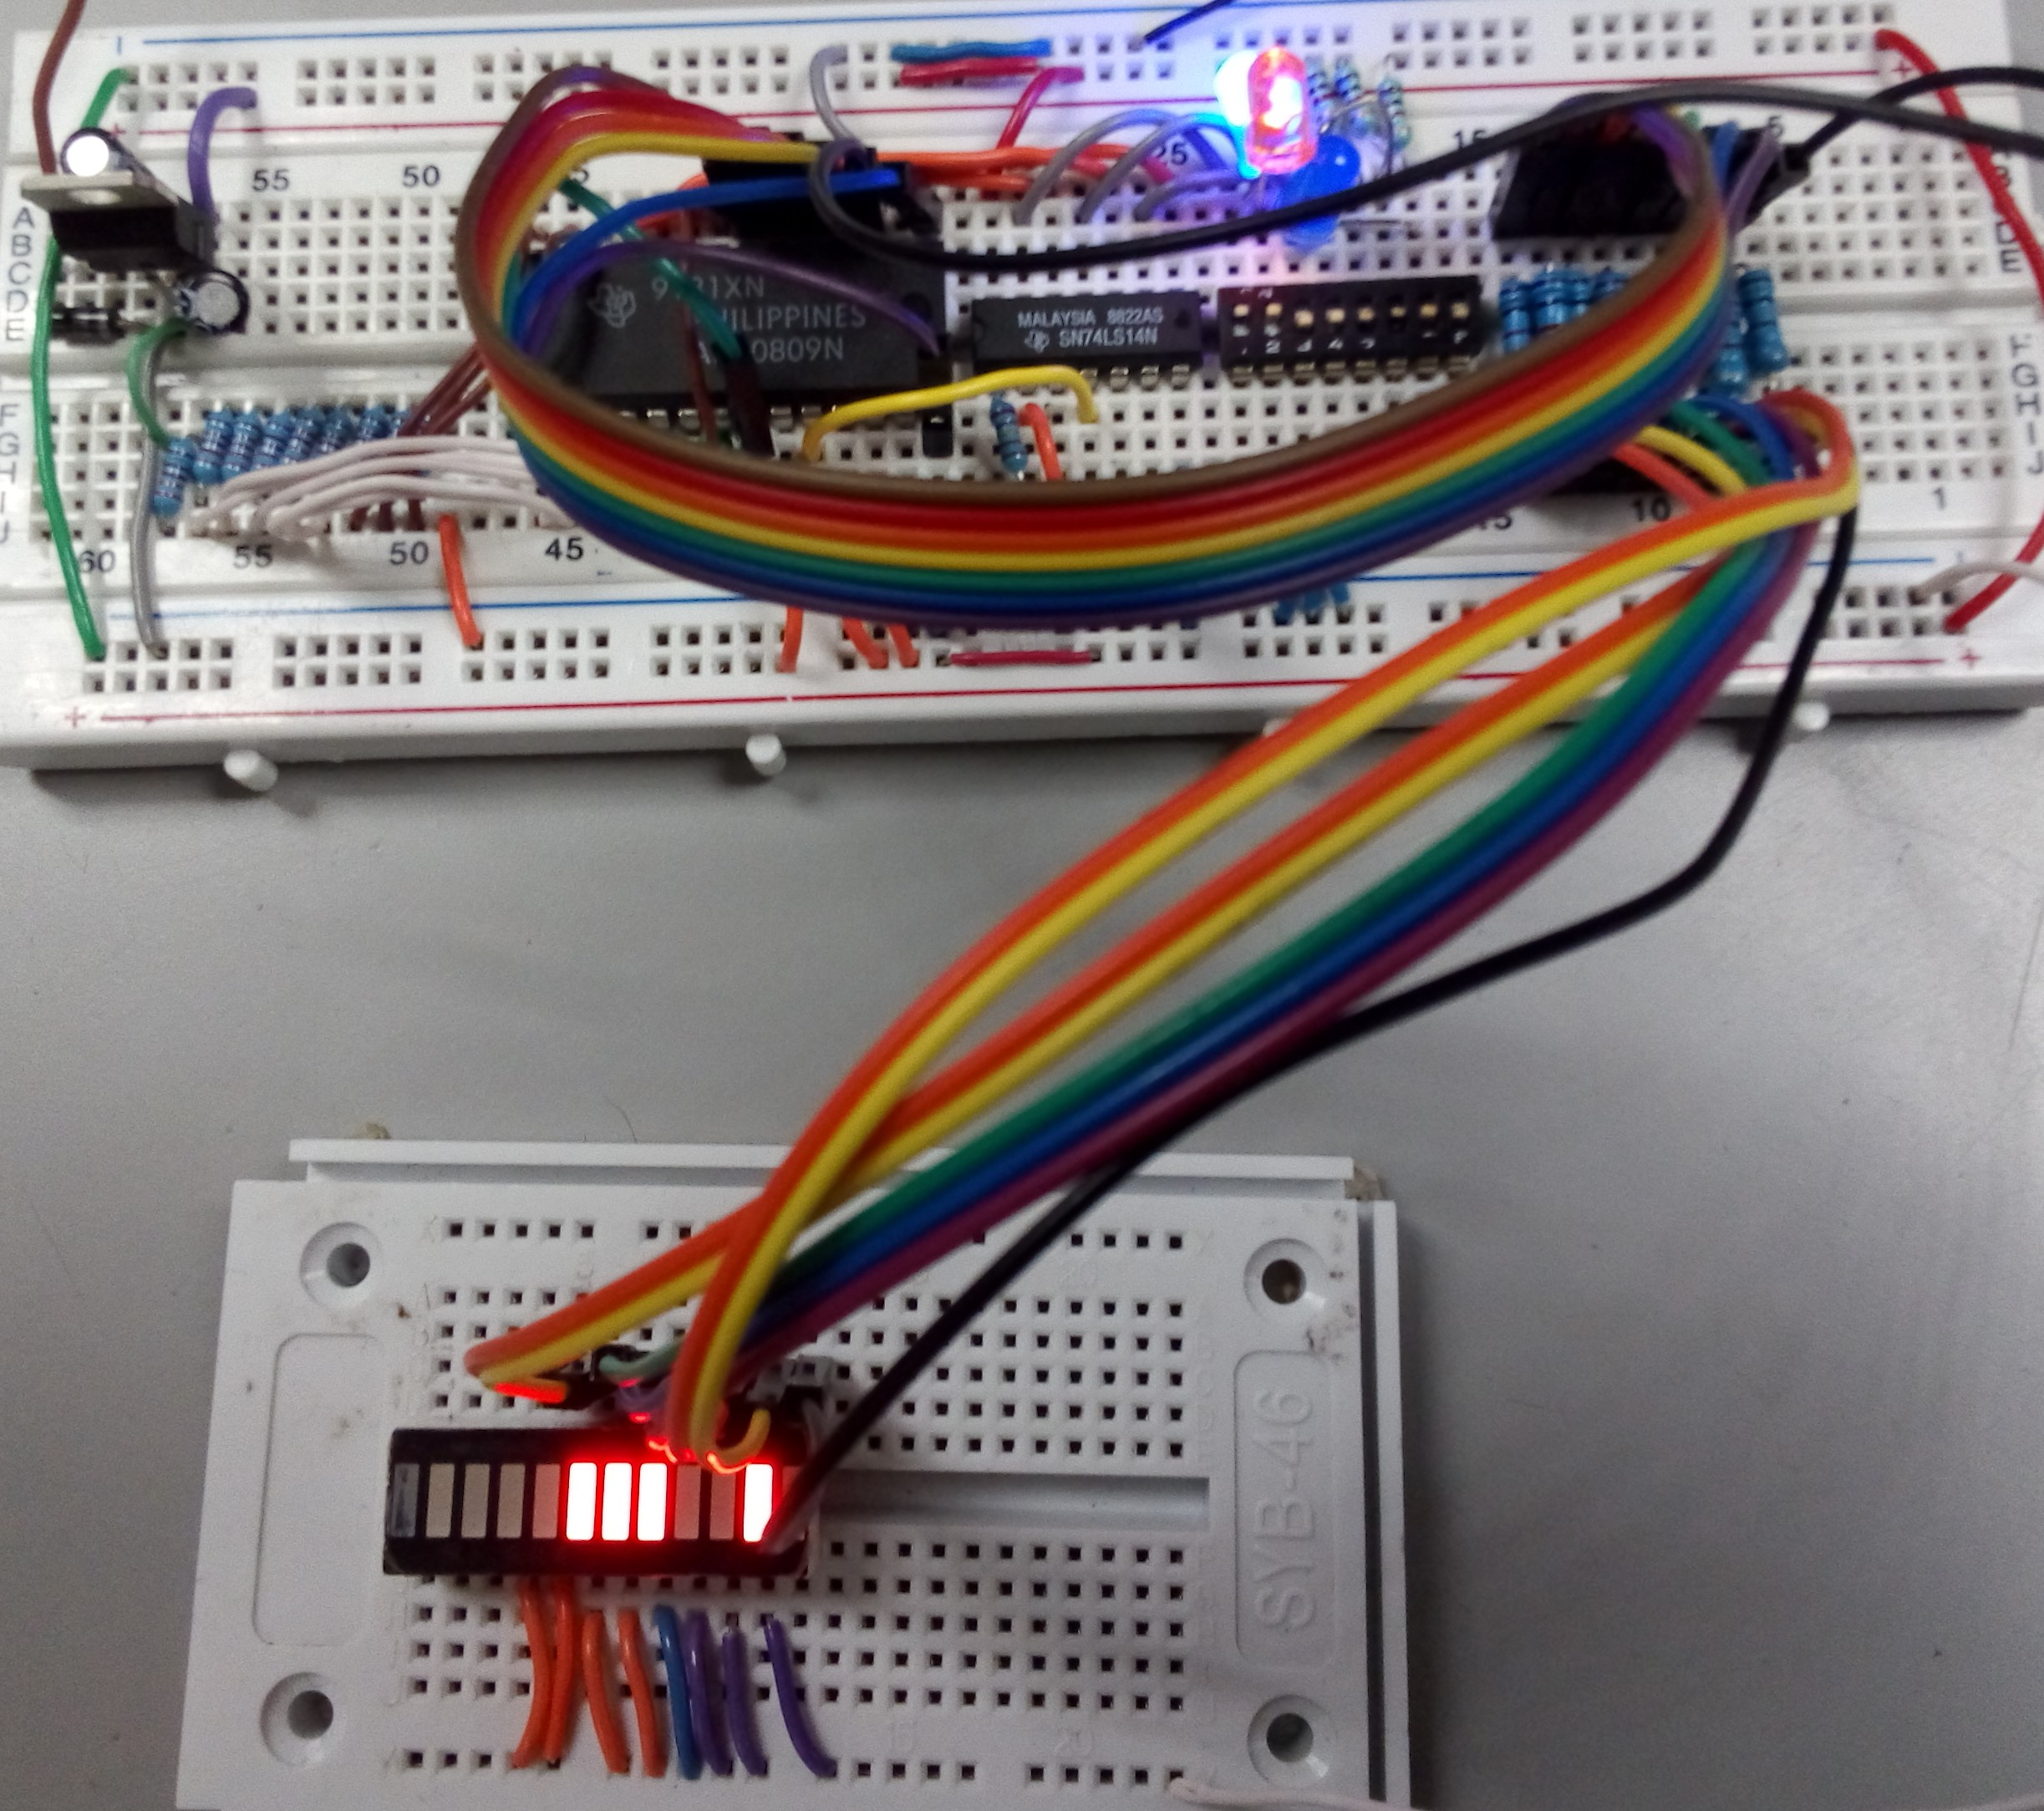
\includegraphics[width=0.69\textwidth]{Practica4/Fotos/canal3_1.jpg}
    \end{figure}
    
    \textbf{Canal 4}
    \begin{figure}[h!]
                \centering
                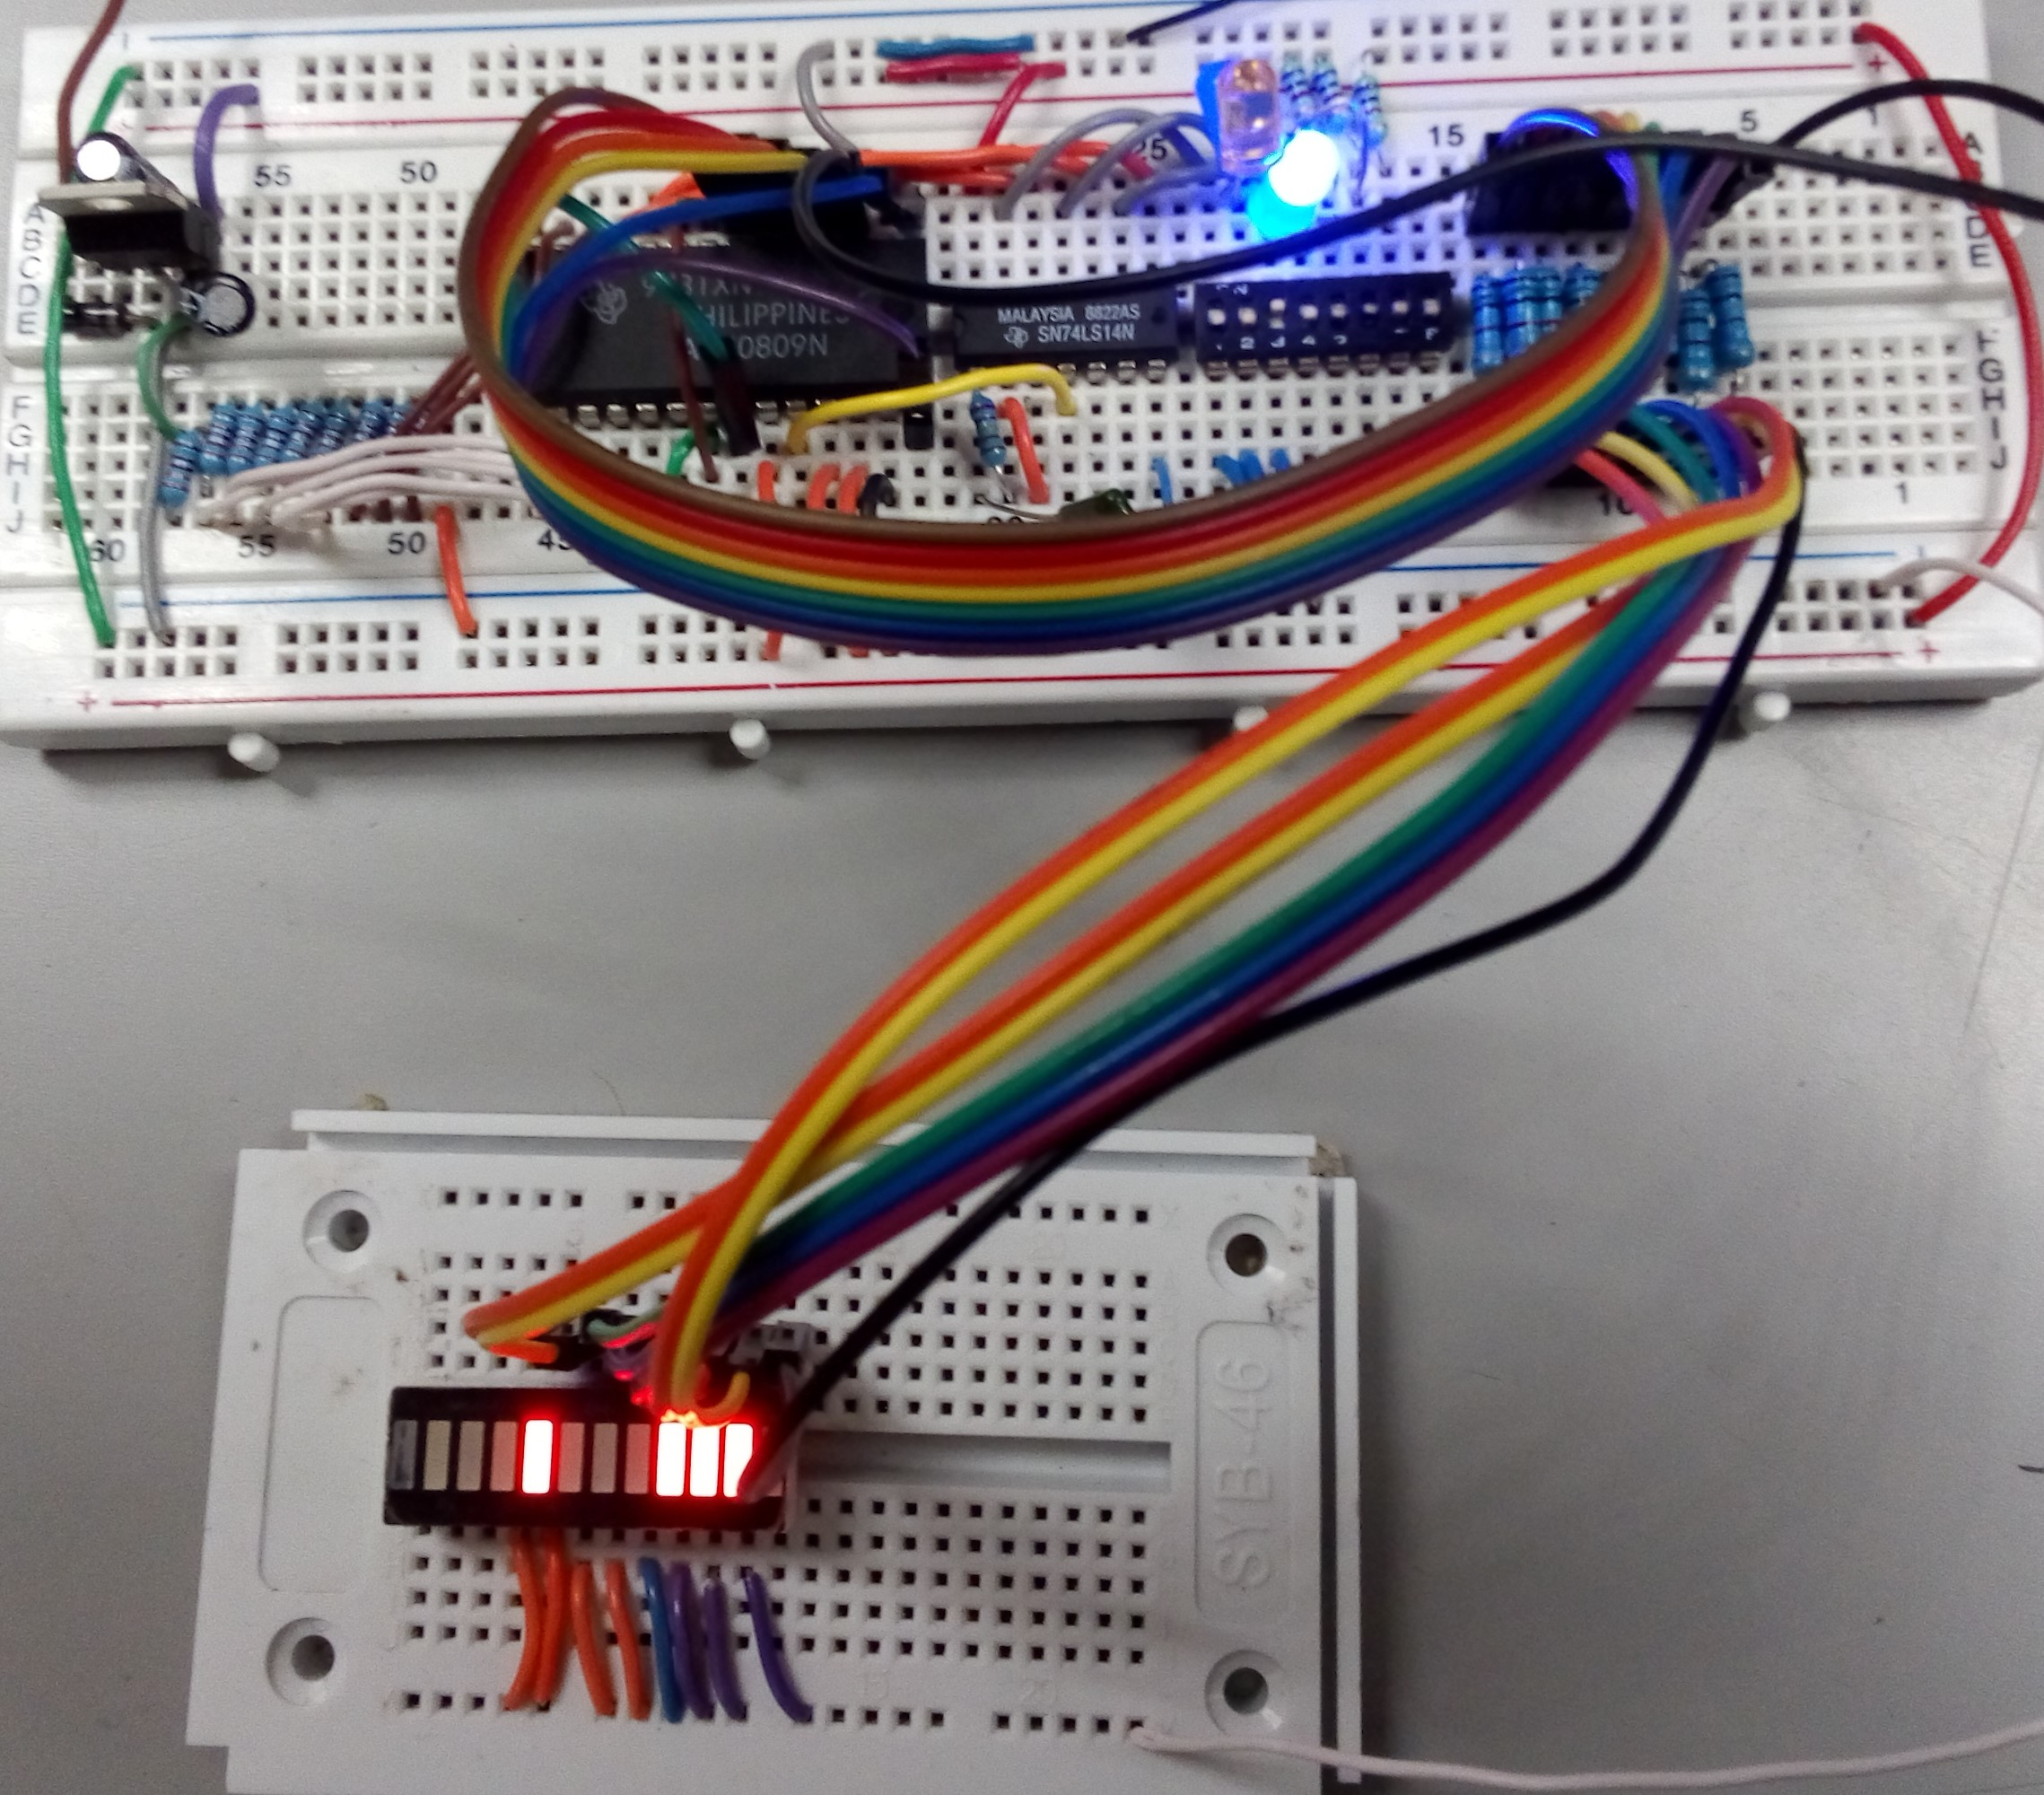
\includegraphics[width=0.69\textwidth]{Practica4/Fotos/canal4_1.jpg}
    \end{figure}
    
    \newpage
    \textbf{Canal 5}
    \begin{figure}[h!]
                \centering
                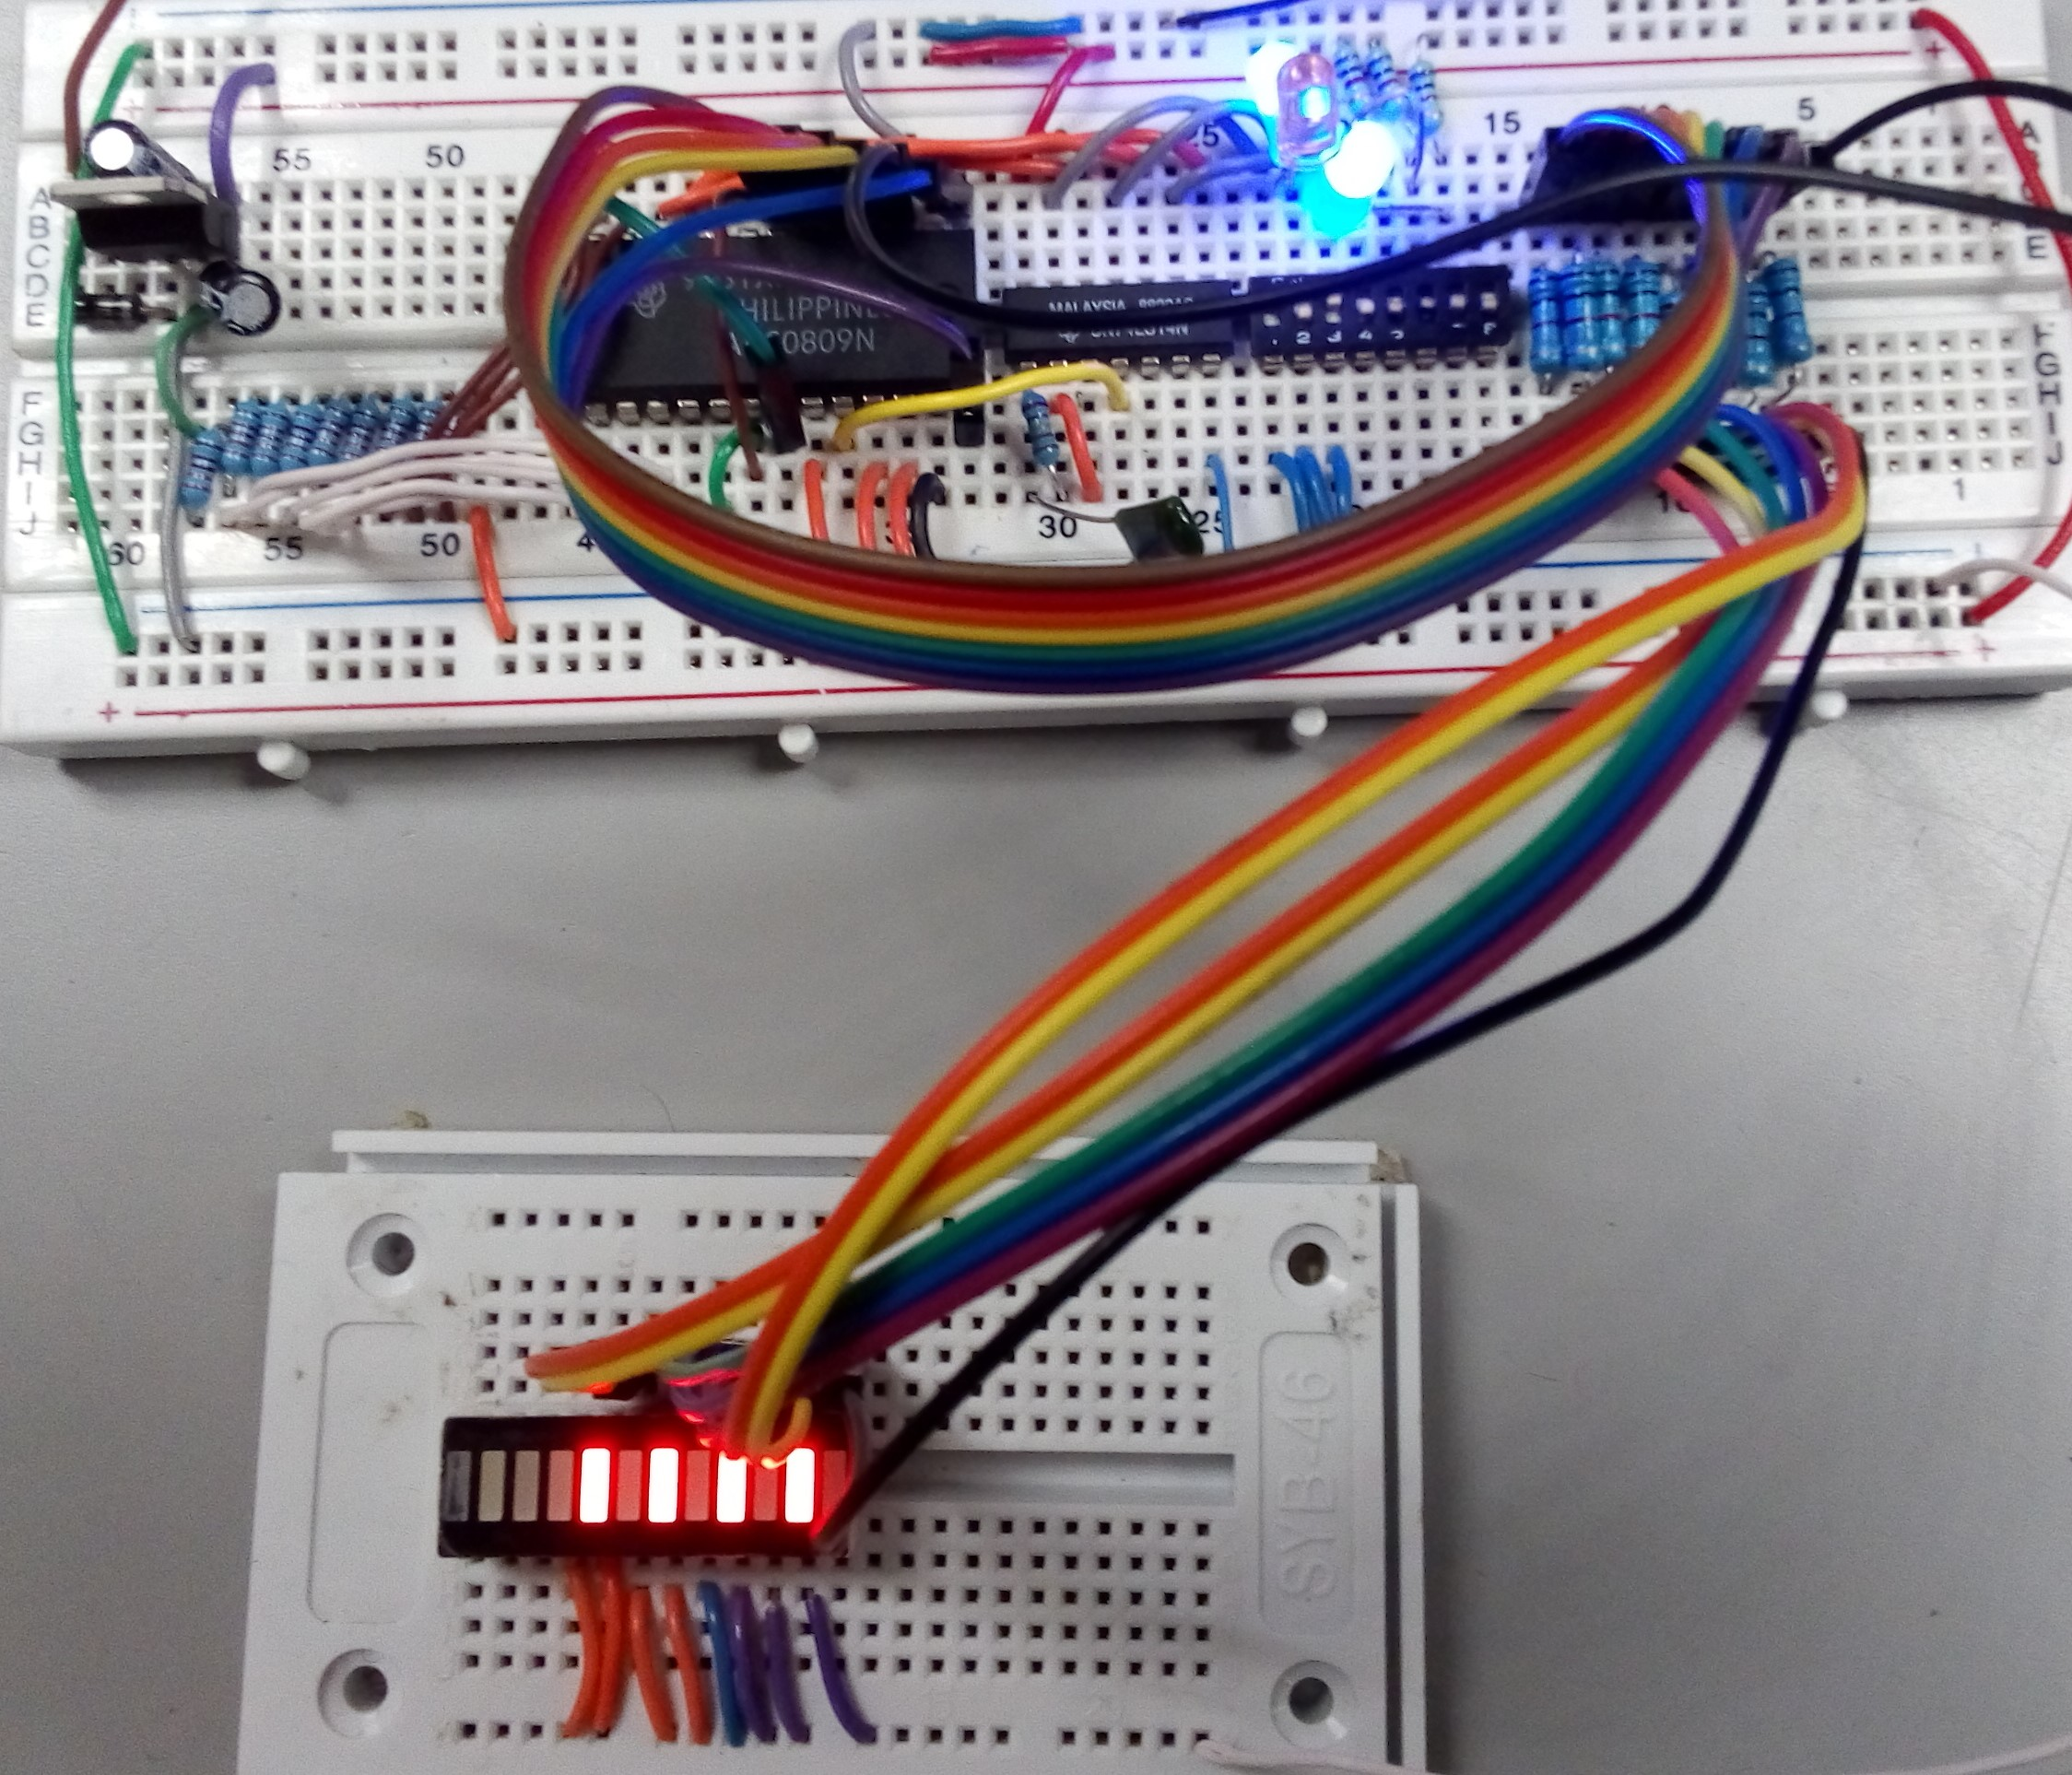
\includegraphics[width=0.69\textwidth]{Practica4/Fotos/canal5_1.jpg}
    \end{figure}
    
    \textbf{Canal 6}
    \begin{figure}[h!]
                \centering
                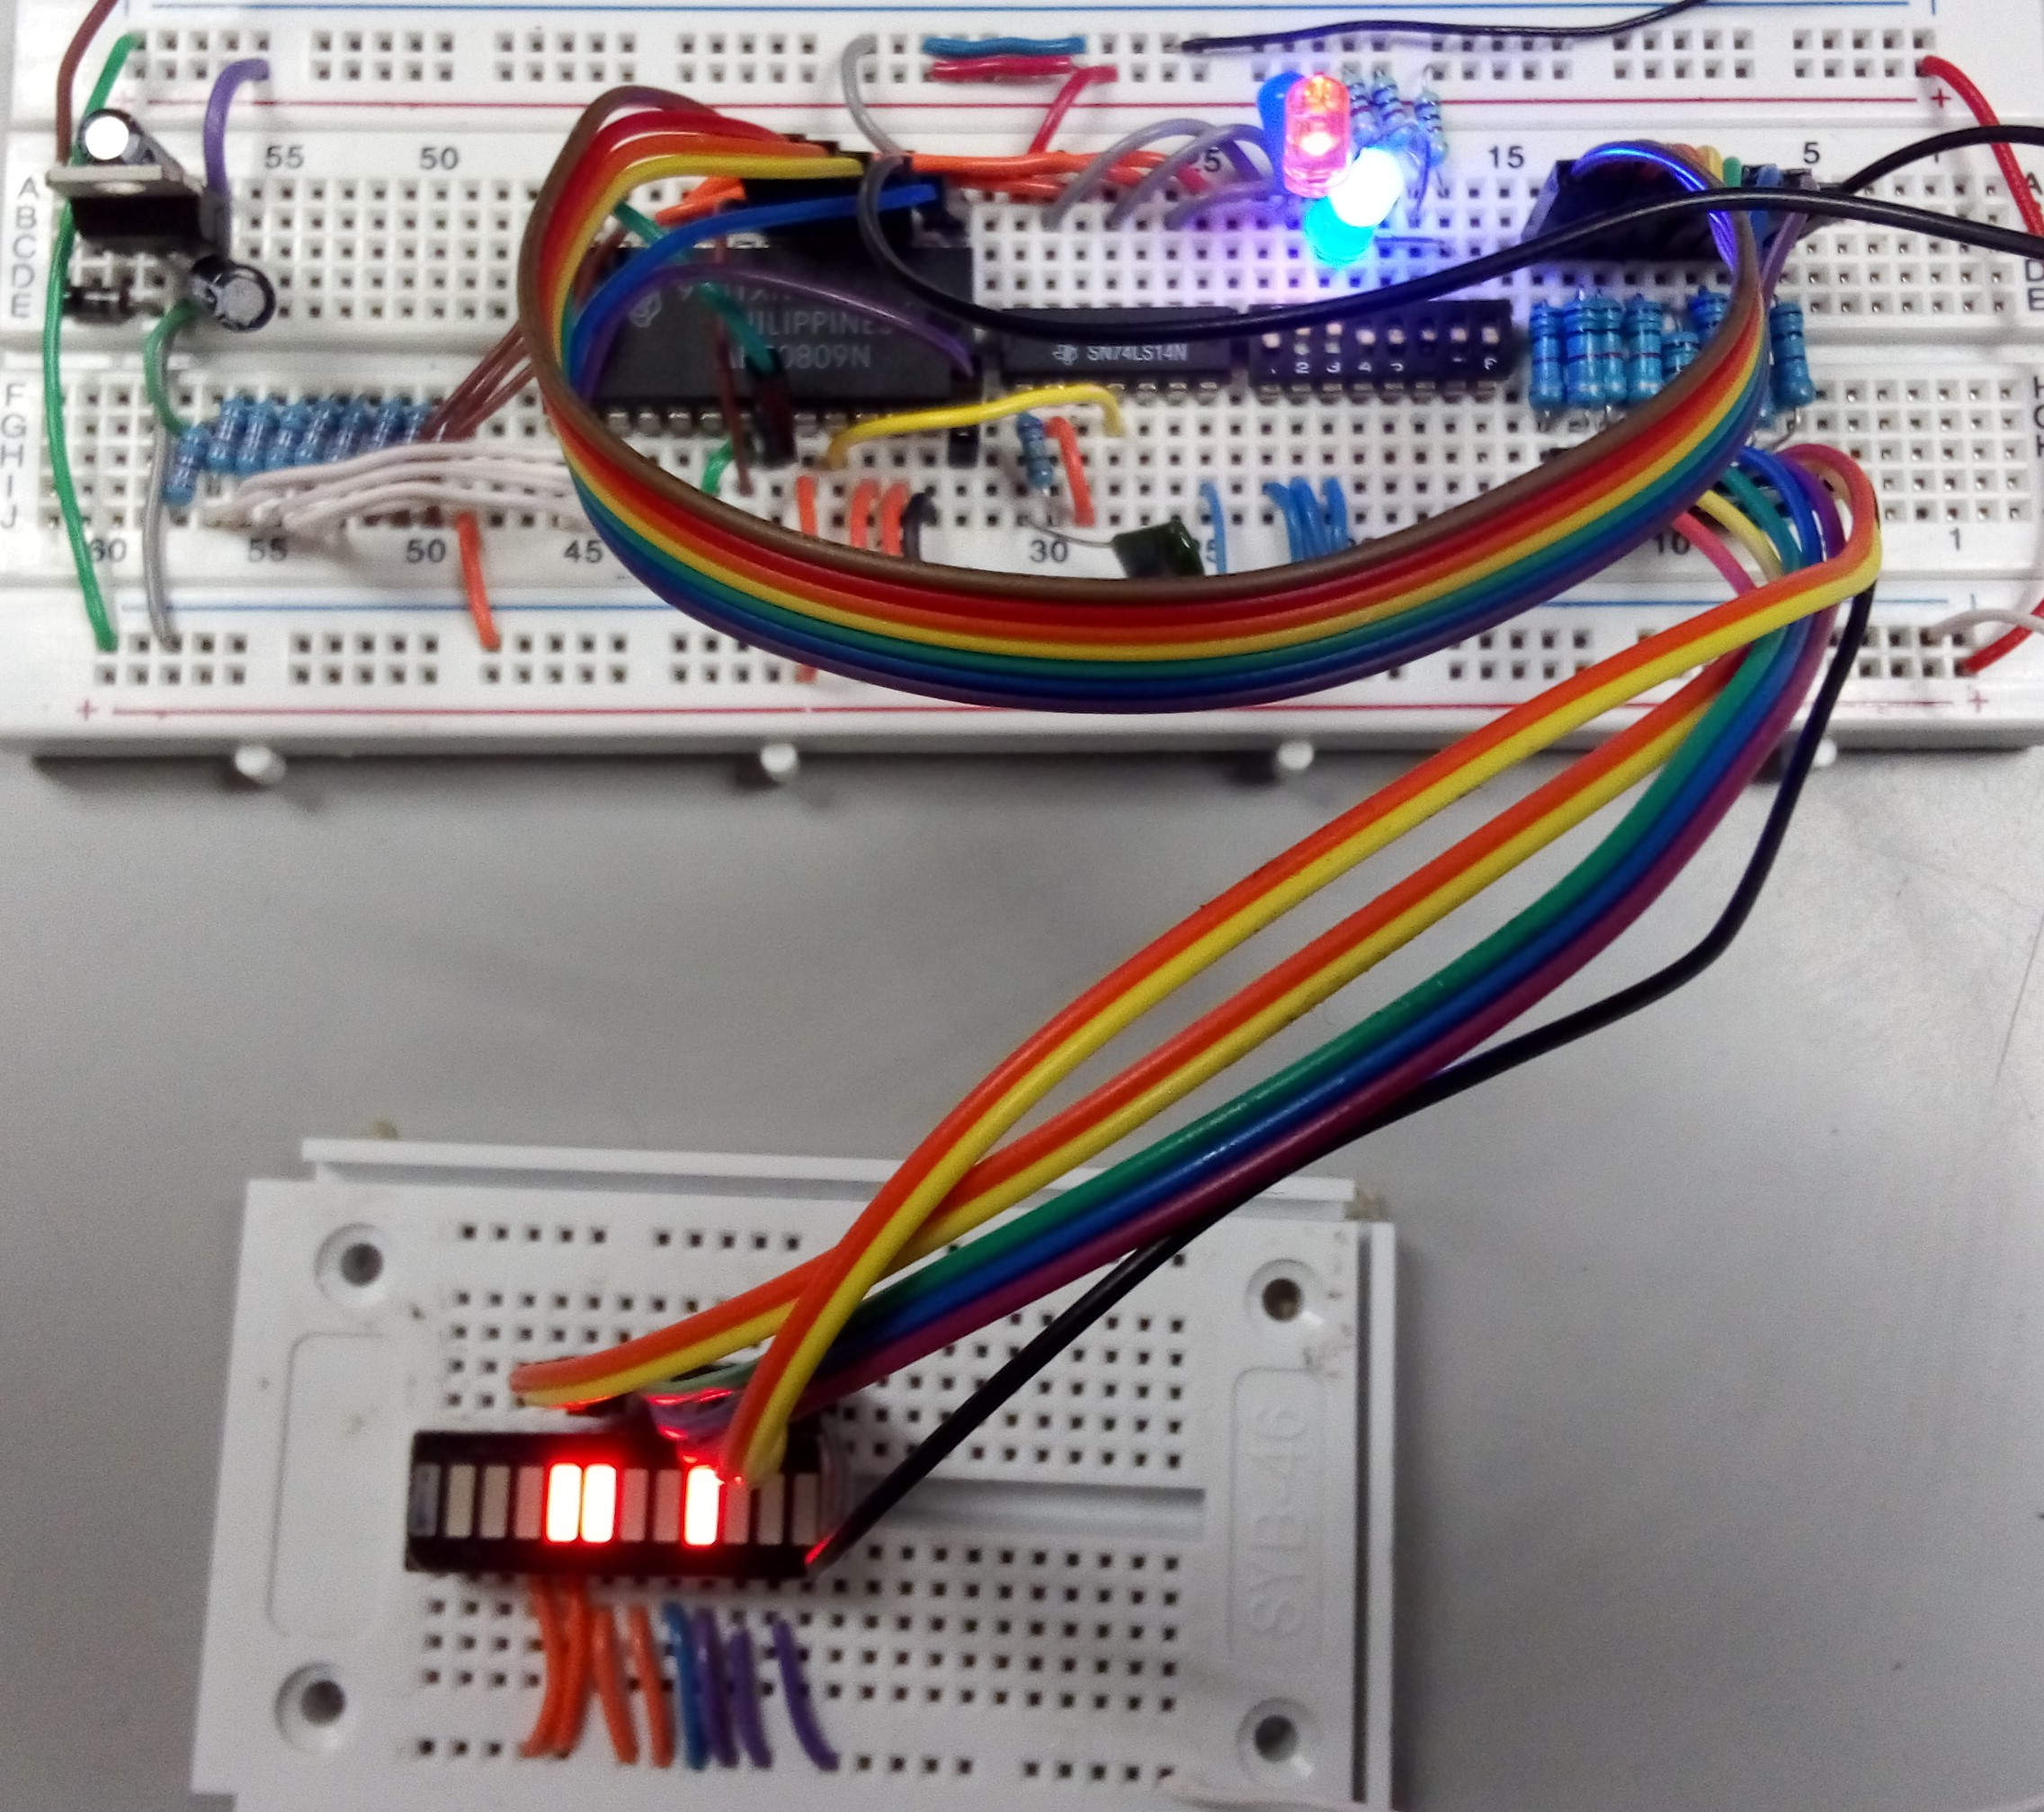
\includegraphics[width=0.69\textwidth]{Practica4/Fotos/canal6_1.jpg}
    \end{figure}
    
    \newpage
    \textbf{Canal 7}
    \begin{figure}[h!]
                \centering
                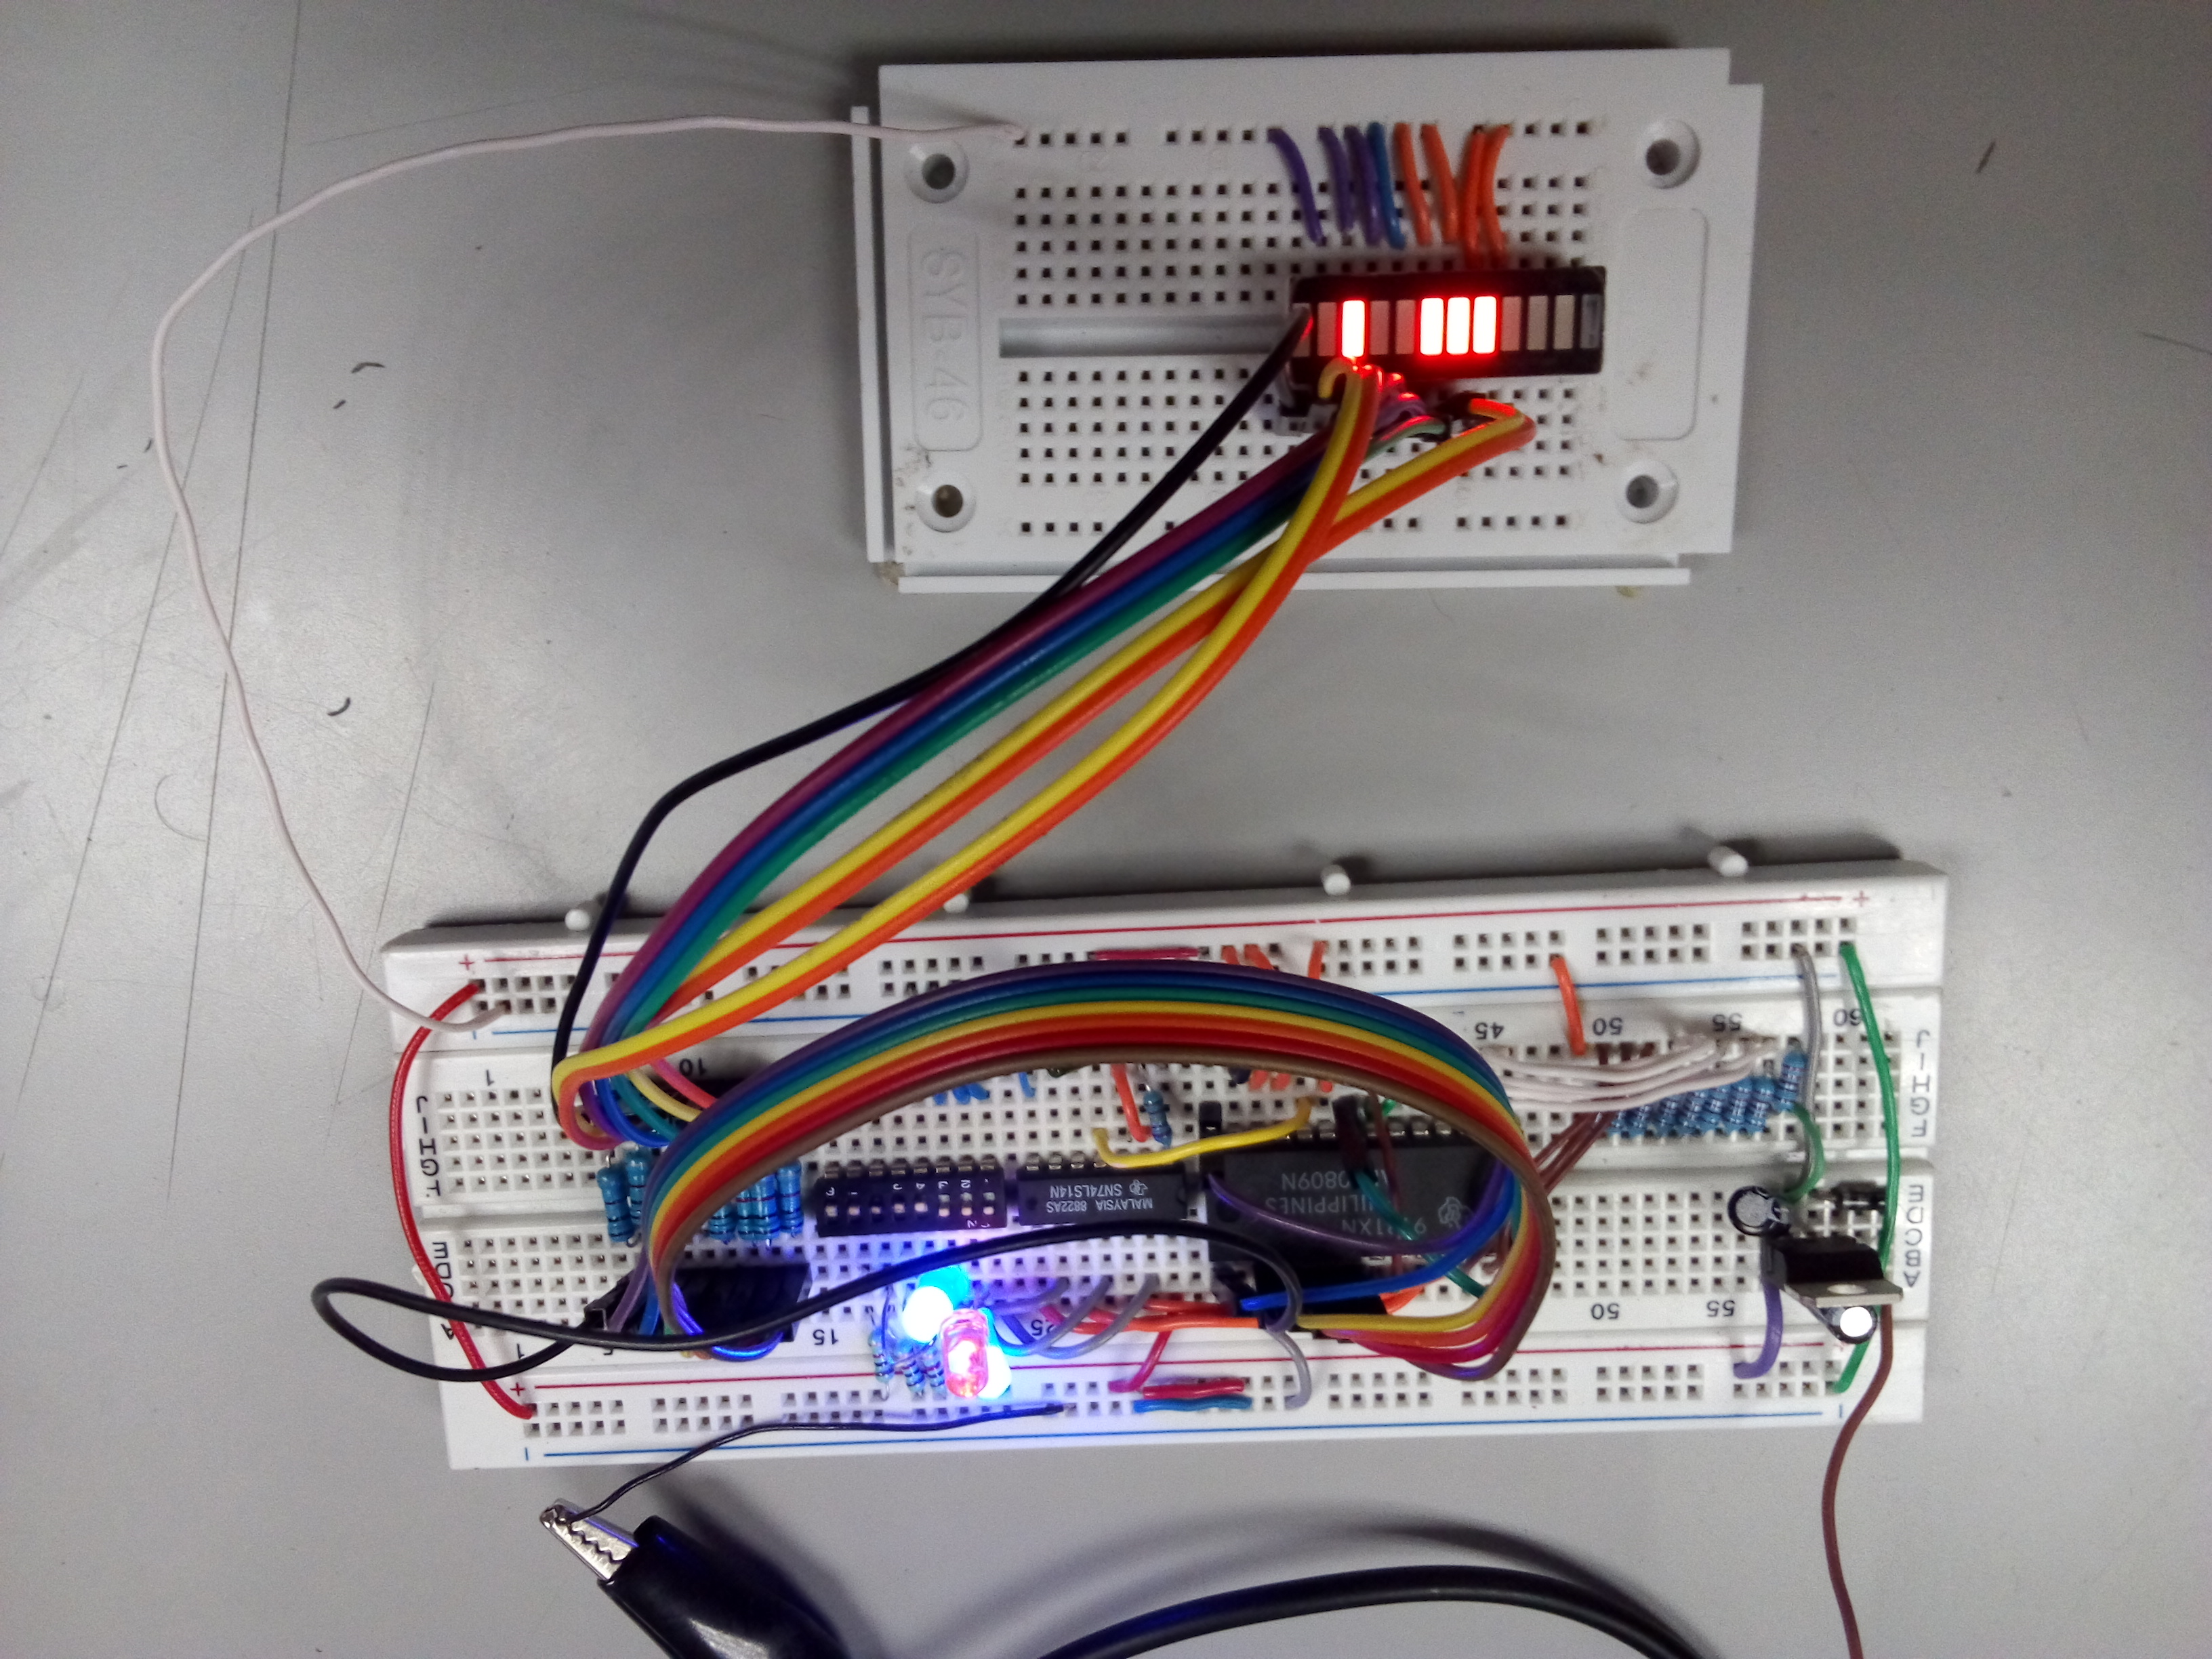
\includegraphics[width=0.71\textwidth]{Practica4/Fotos/canal7.jpg}
    \end{figure}
    
	% ---------------------------------------------------------

	\subsection{PE 3 - Acondicionamiento de la entradas del sensor de temperatura}
	Un tema importante cuando utilizamos un conversor AD es el acondicionamiento de la entrada. Realizaremos el acondicionamiento de una señal proveniente de un sensor de temperatura LM35. Este sensor entrega 10mV/$^{\circ}$C, con lo que a 100ºC entrega 1V.

    Supondremos que mediremos la temperatura ambiente por lo que estableceremos la temperatura máxima en 50 grados centígrados a plena escala (es decir, 500 mV como salida máxima del sensor, y voltaje de entrada al amplificador). De acuerdo a esto calcule la ganancia y los componentes necesarios para que a 50 grados centígrados el voltaje a la salida de la etapa de acondicionamiento tengamos 5V.
    
    \begin{figure}[h!]
                \centering
                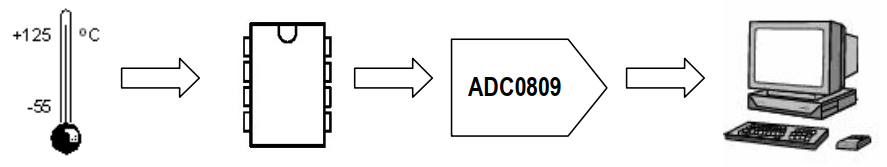
\includegraphics[width=\textwidth]{Practica4/Images/img6.PNG}
    \end{figure}
    \newpage
	\subsubsection{Esquema}
	\begin{figure}[h!]
                \centering
                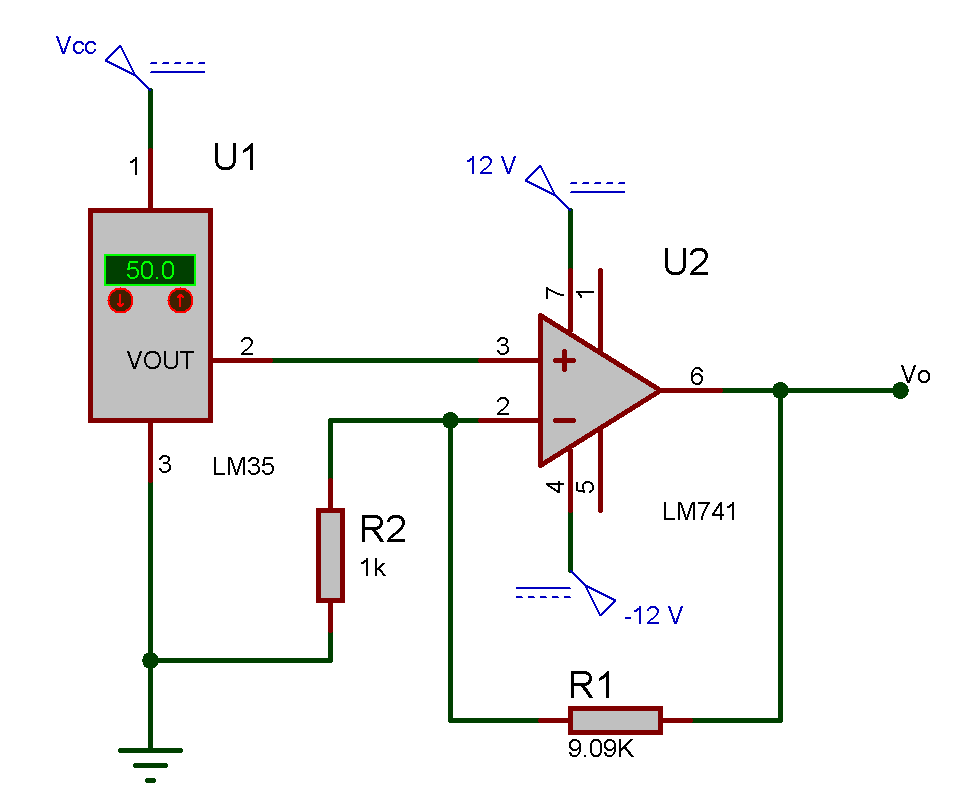
\includegraphics[width=0.7\textwidth]{Practica4/Images/temperatura.png}
    \end{figure}
	\subsubsection{Circuito cableado}
	\begin{figure}[h!]
                \centering
                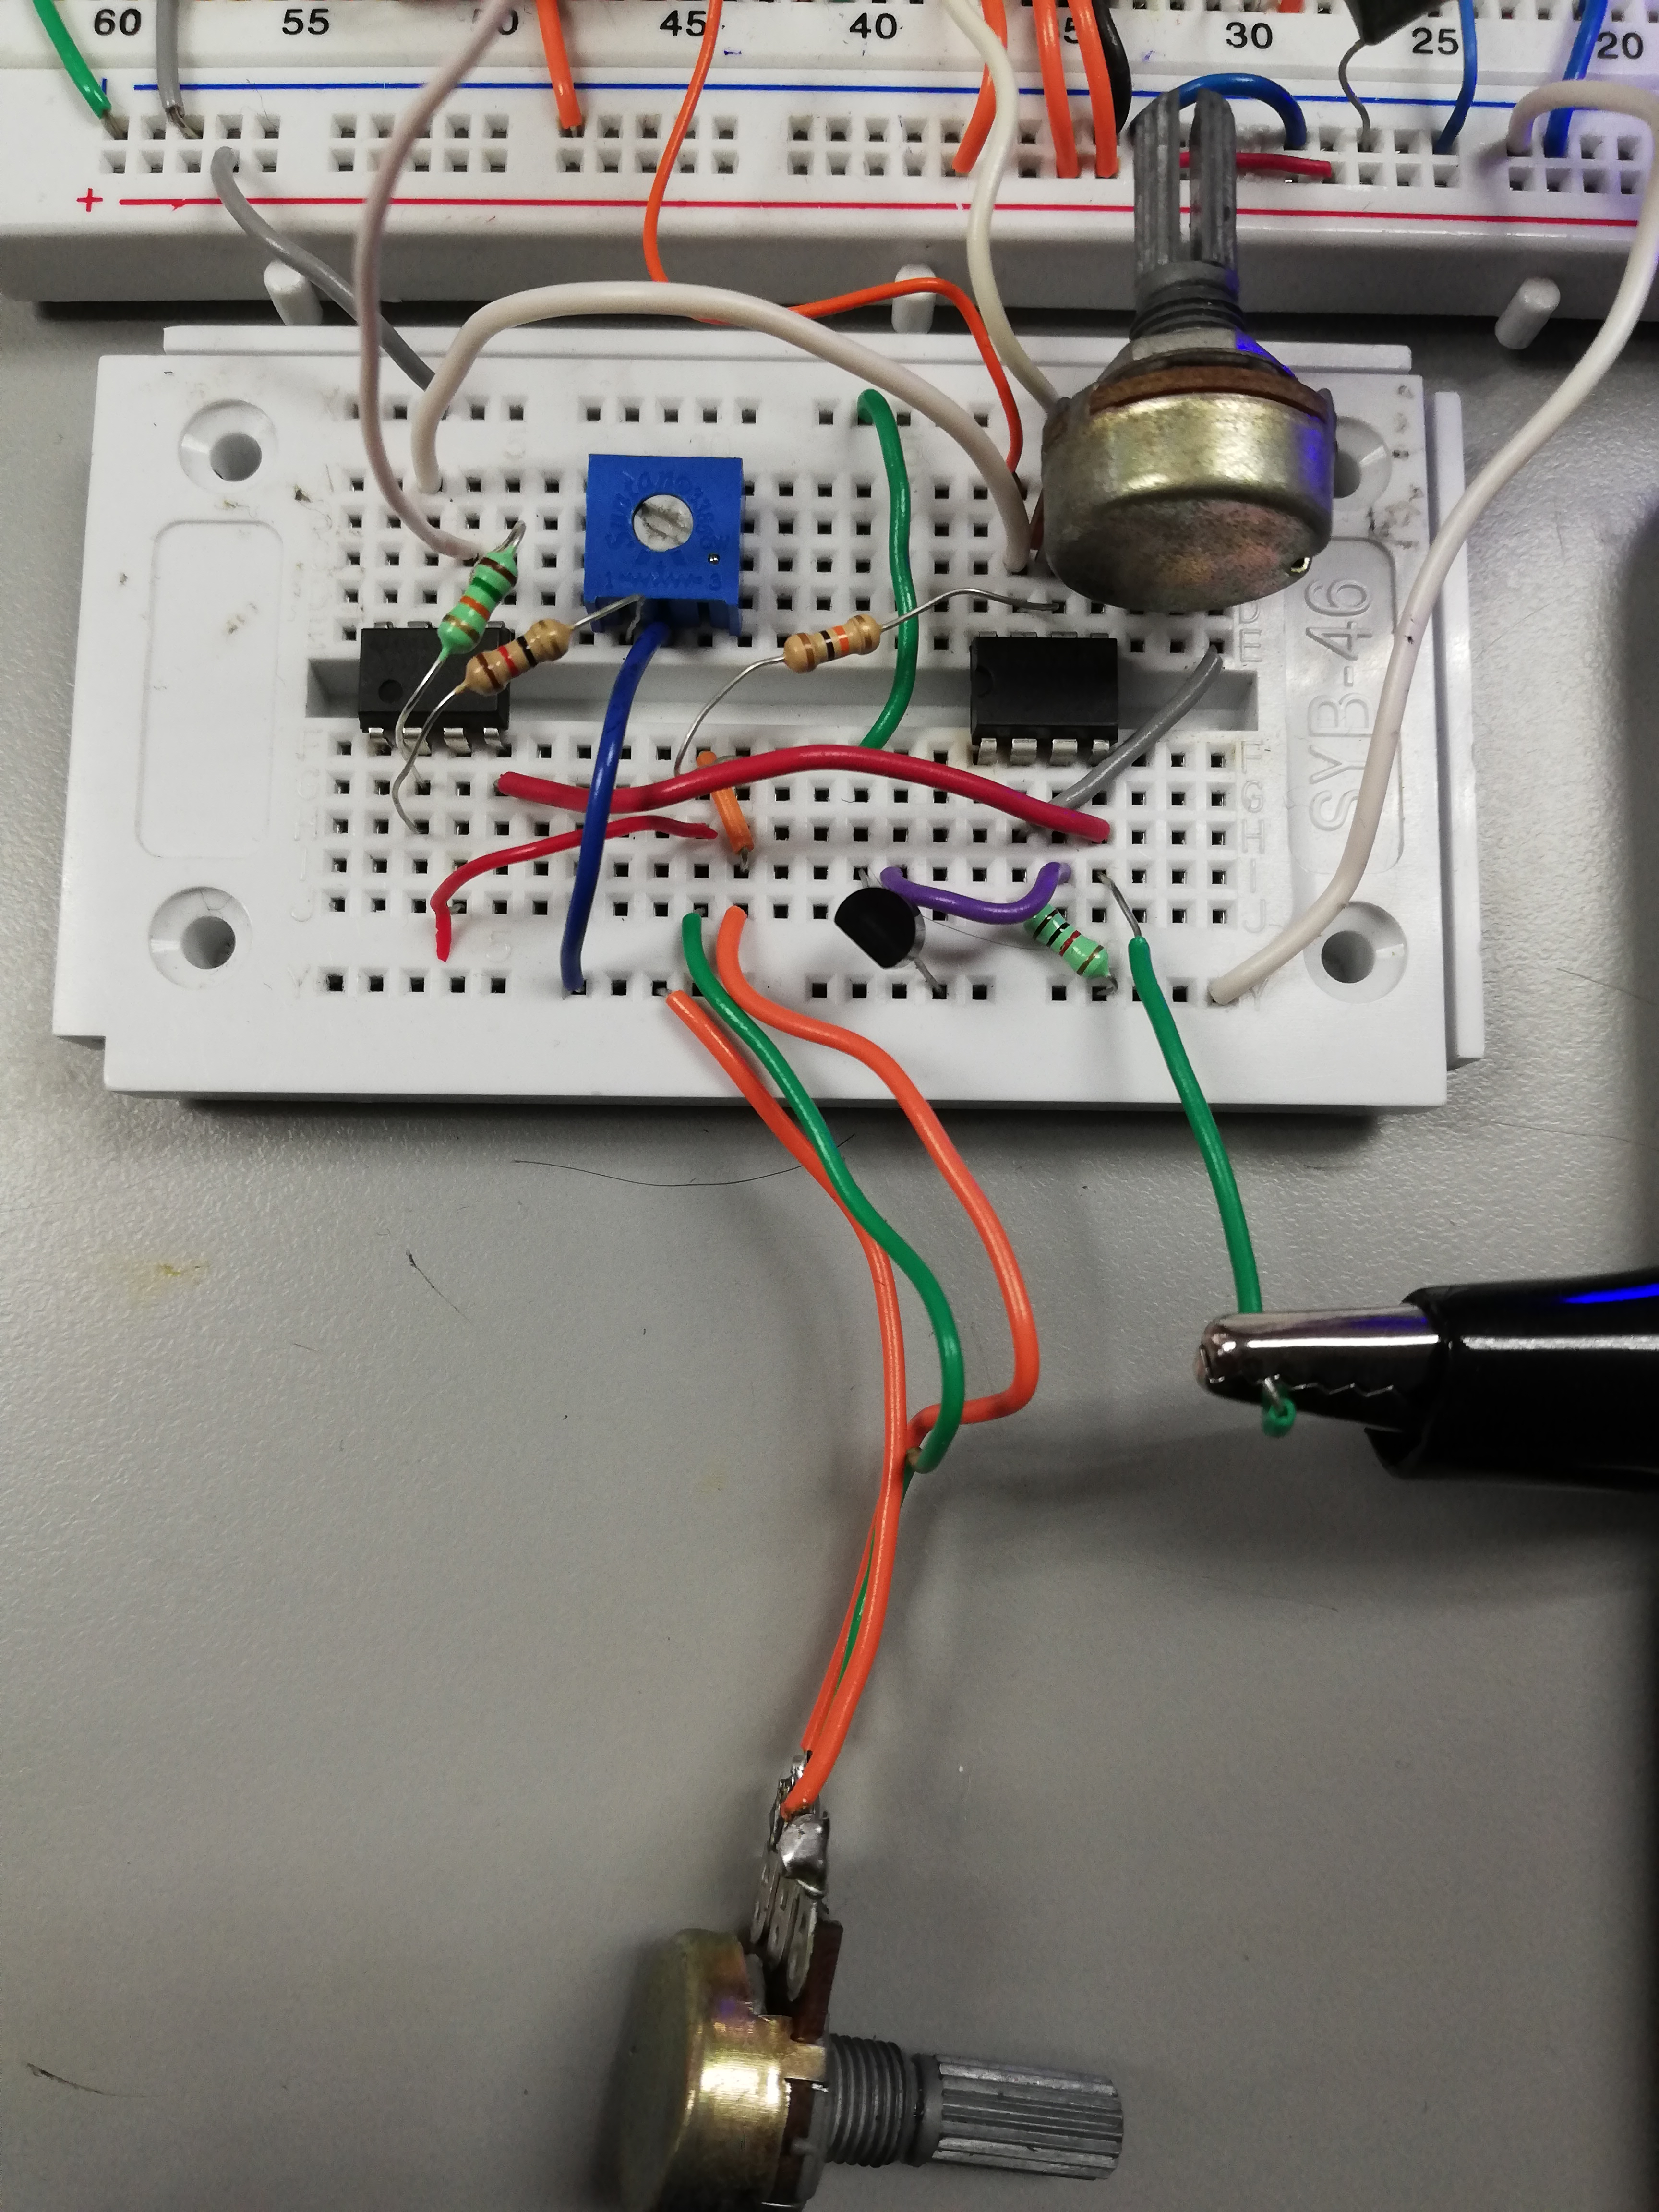
\includegraphics[width=0.75\textwidth]{Practica4/Fotos/sensor2.jpg}
    \end{figure}
    
	\subsubsection{Funcionamiento}
	La salida $V_{o}$ del circuito (salida 6 del amplificador) la enviamos al Canal 0 del convertidor ADC0809. 
	
	Seleccionamos en el dipswitch este canal y observamos. Notamos que en la tira de LEDs el valor binario va aumentando o disminuyendo; esto depende mucho de la temperatura ambiente al momento de conectar el circuito.
	
	Cuando colocamos, por ejemplo, los dedos alrededor del sensor LM35, el valor binario empieza a aumentar de uno en uno, poco a poco. Una vez que soltamos el sensor, este empieza a bajar nuevamente hasta estabilizarse en algún valor específico.
	
	\begin{figure}[h!]
                \centering
                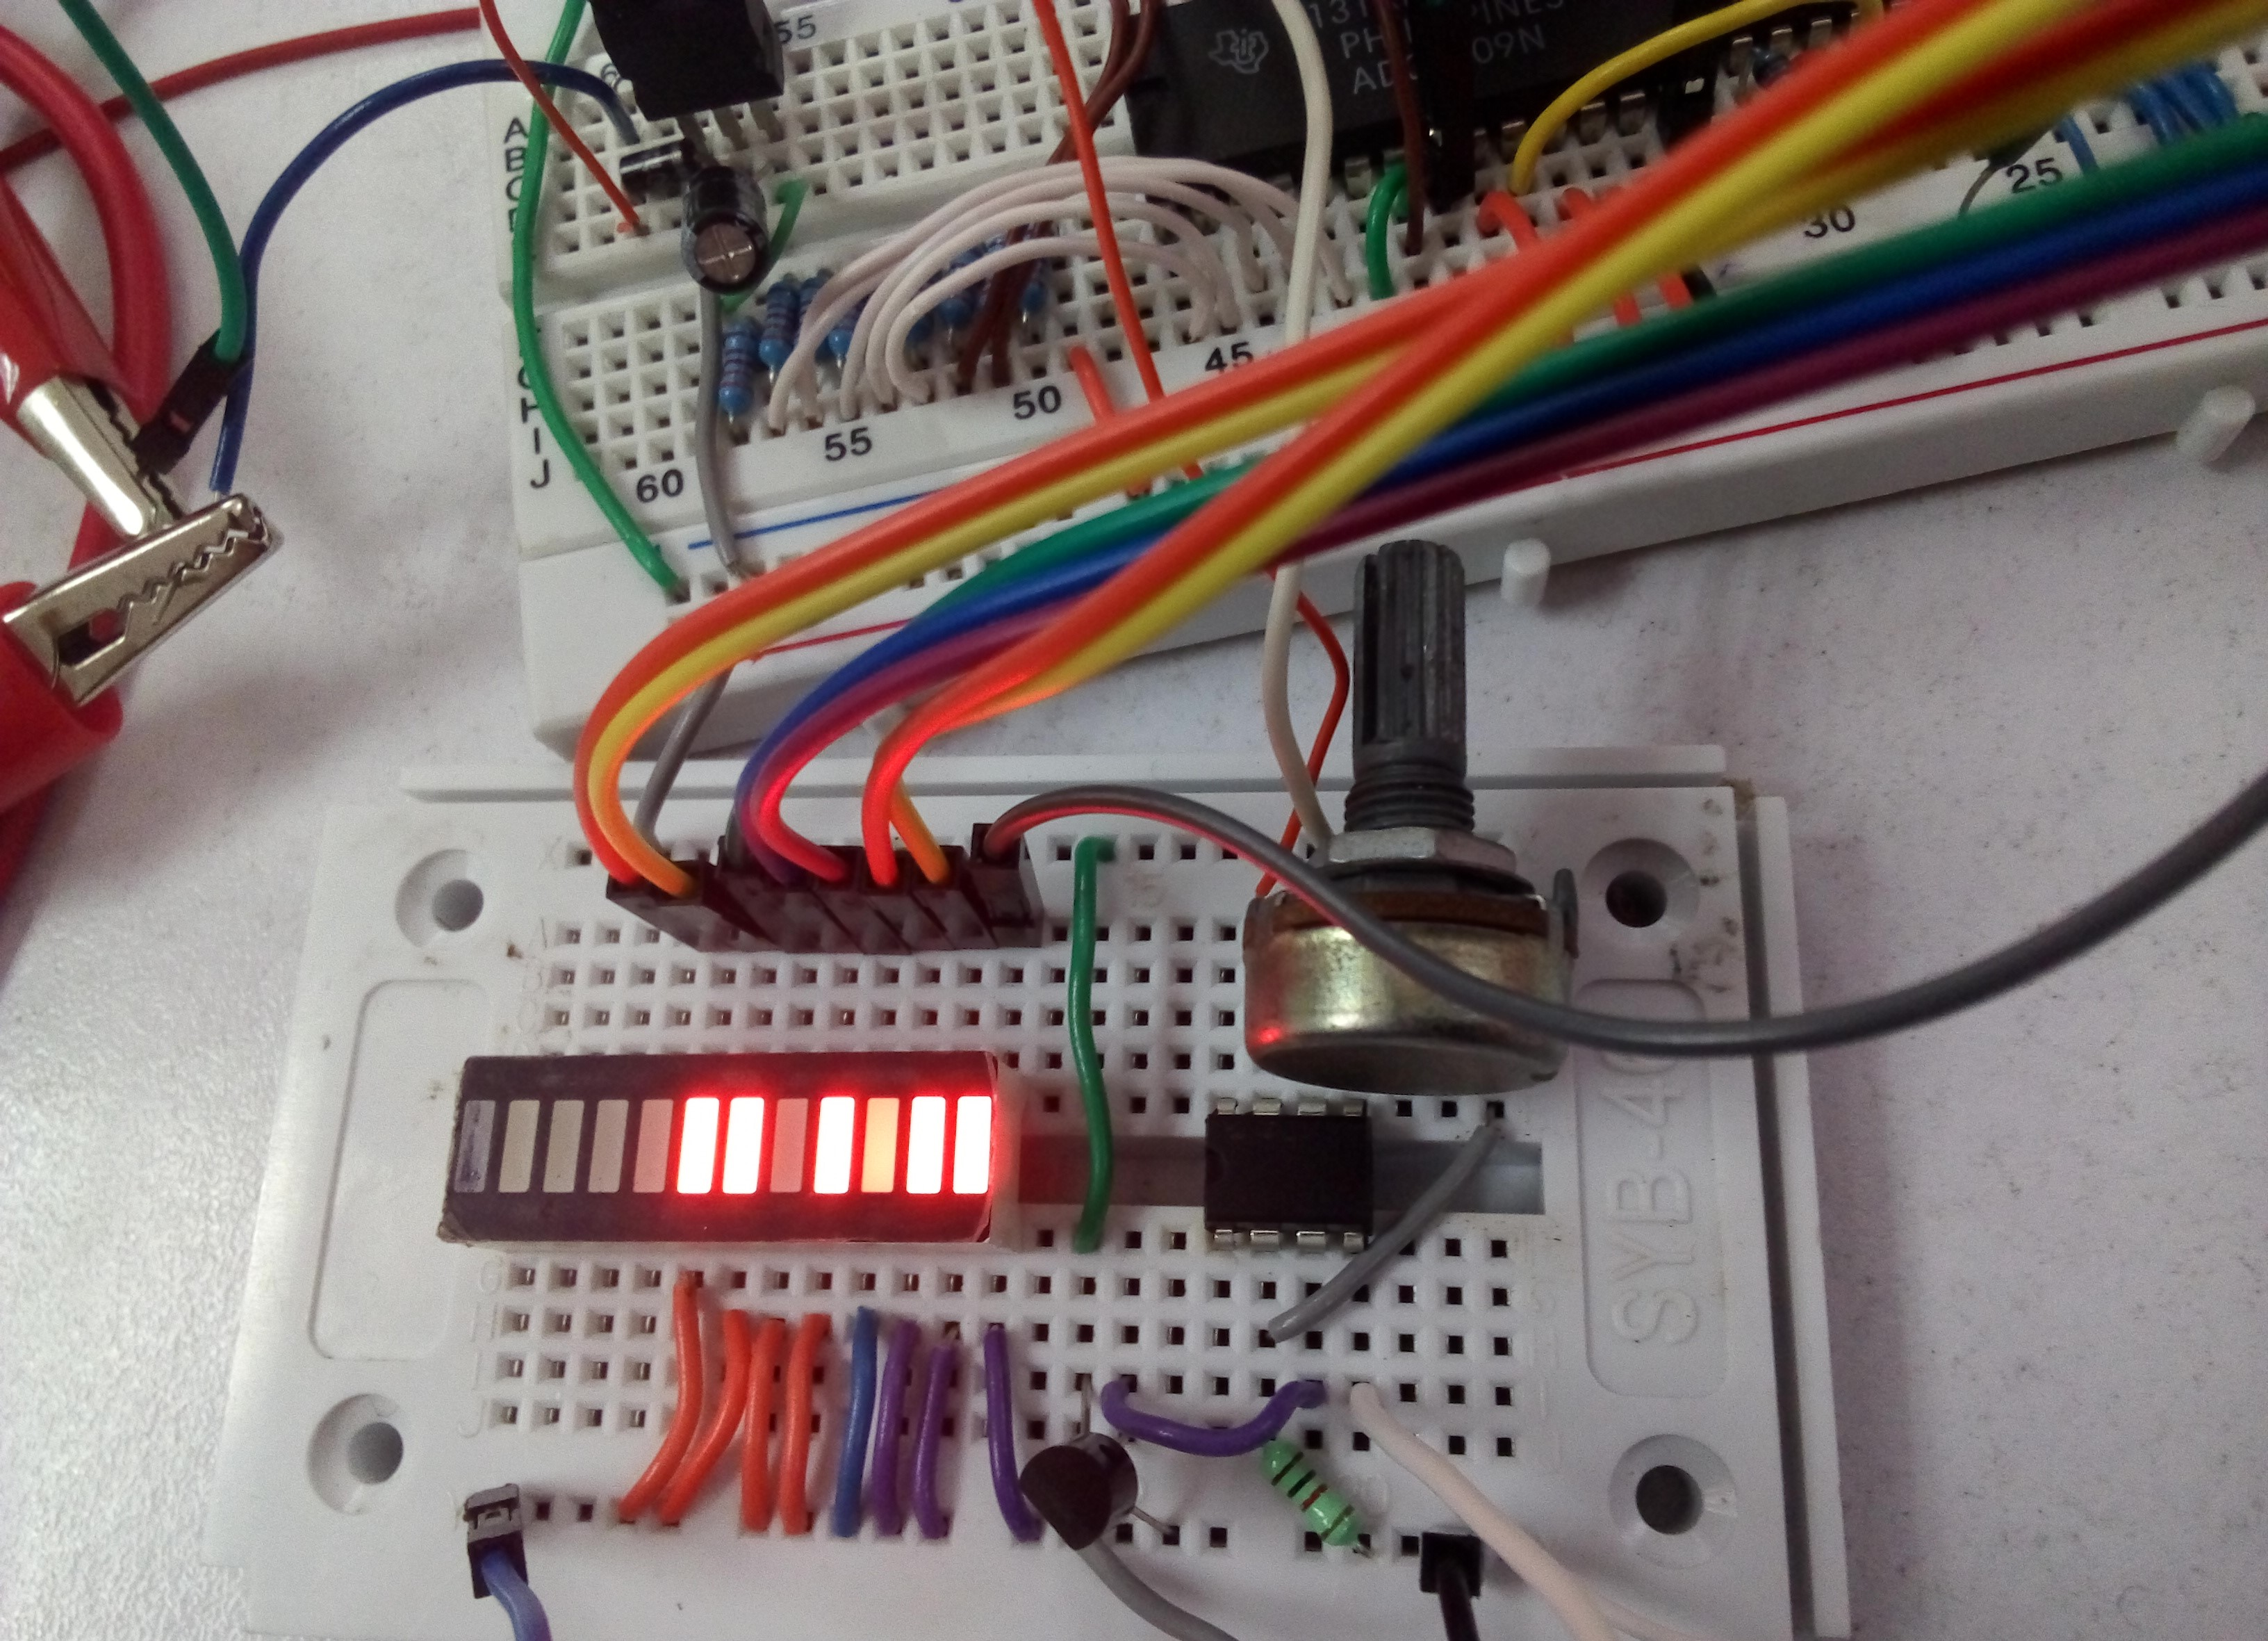
\includegraphics[width=0.68\textwidth]{Practica4/Fotos/temperatura3.jpg}
    \end{figure}

    \begin{figure}[h!]
                \centering
                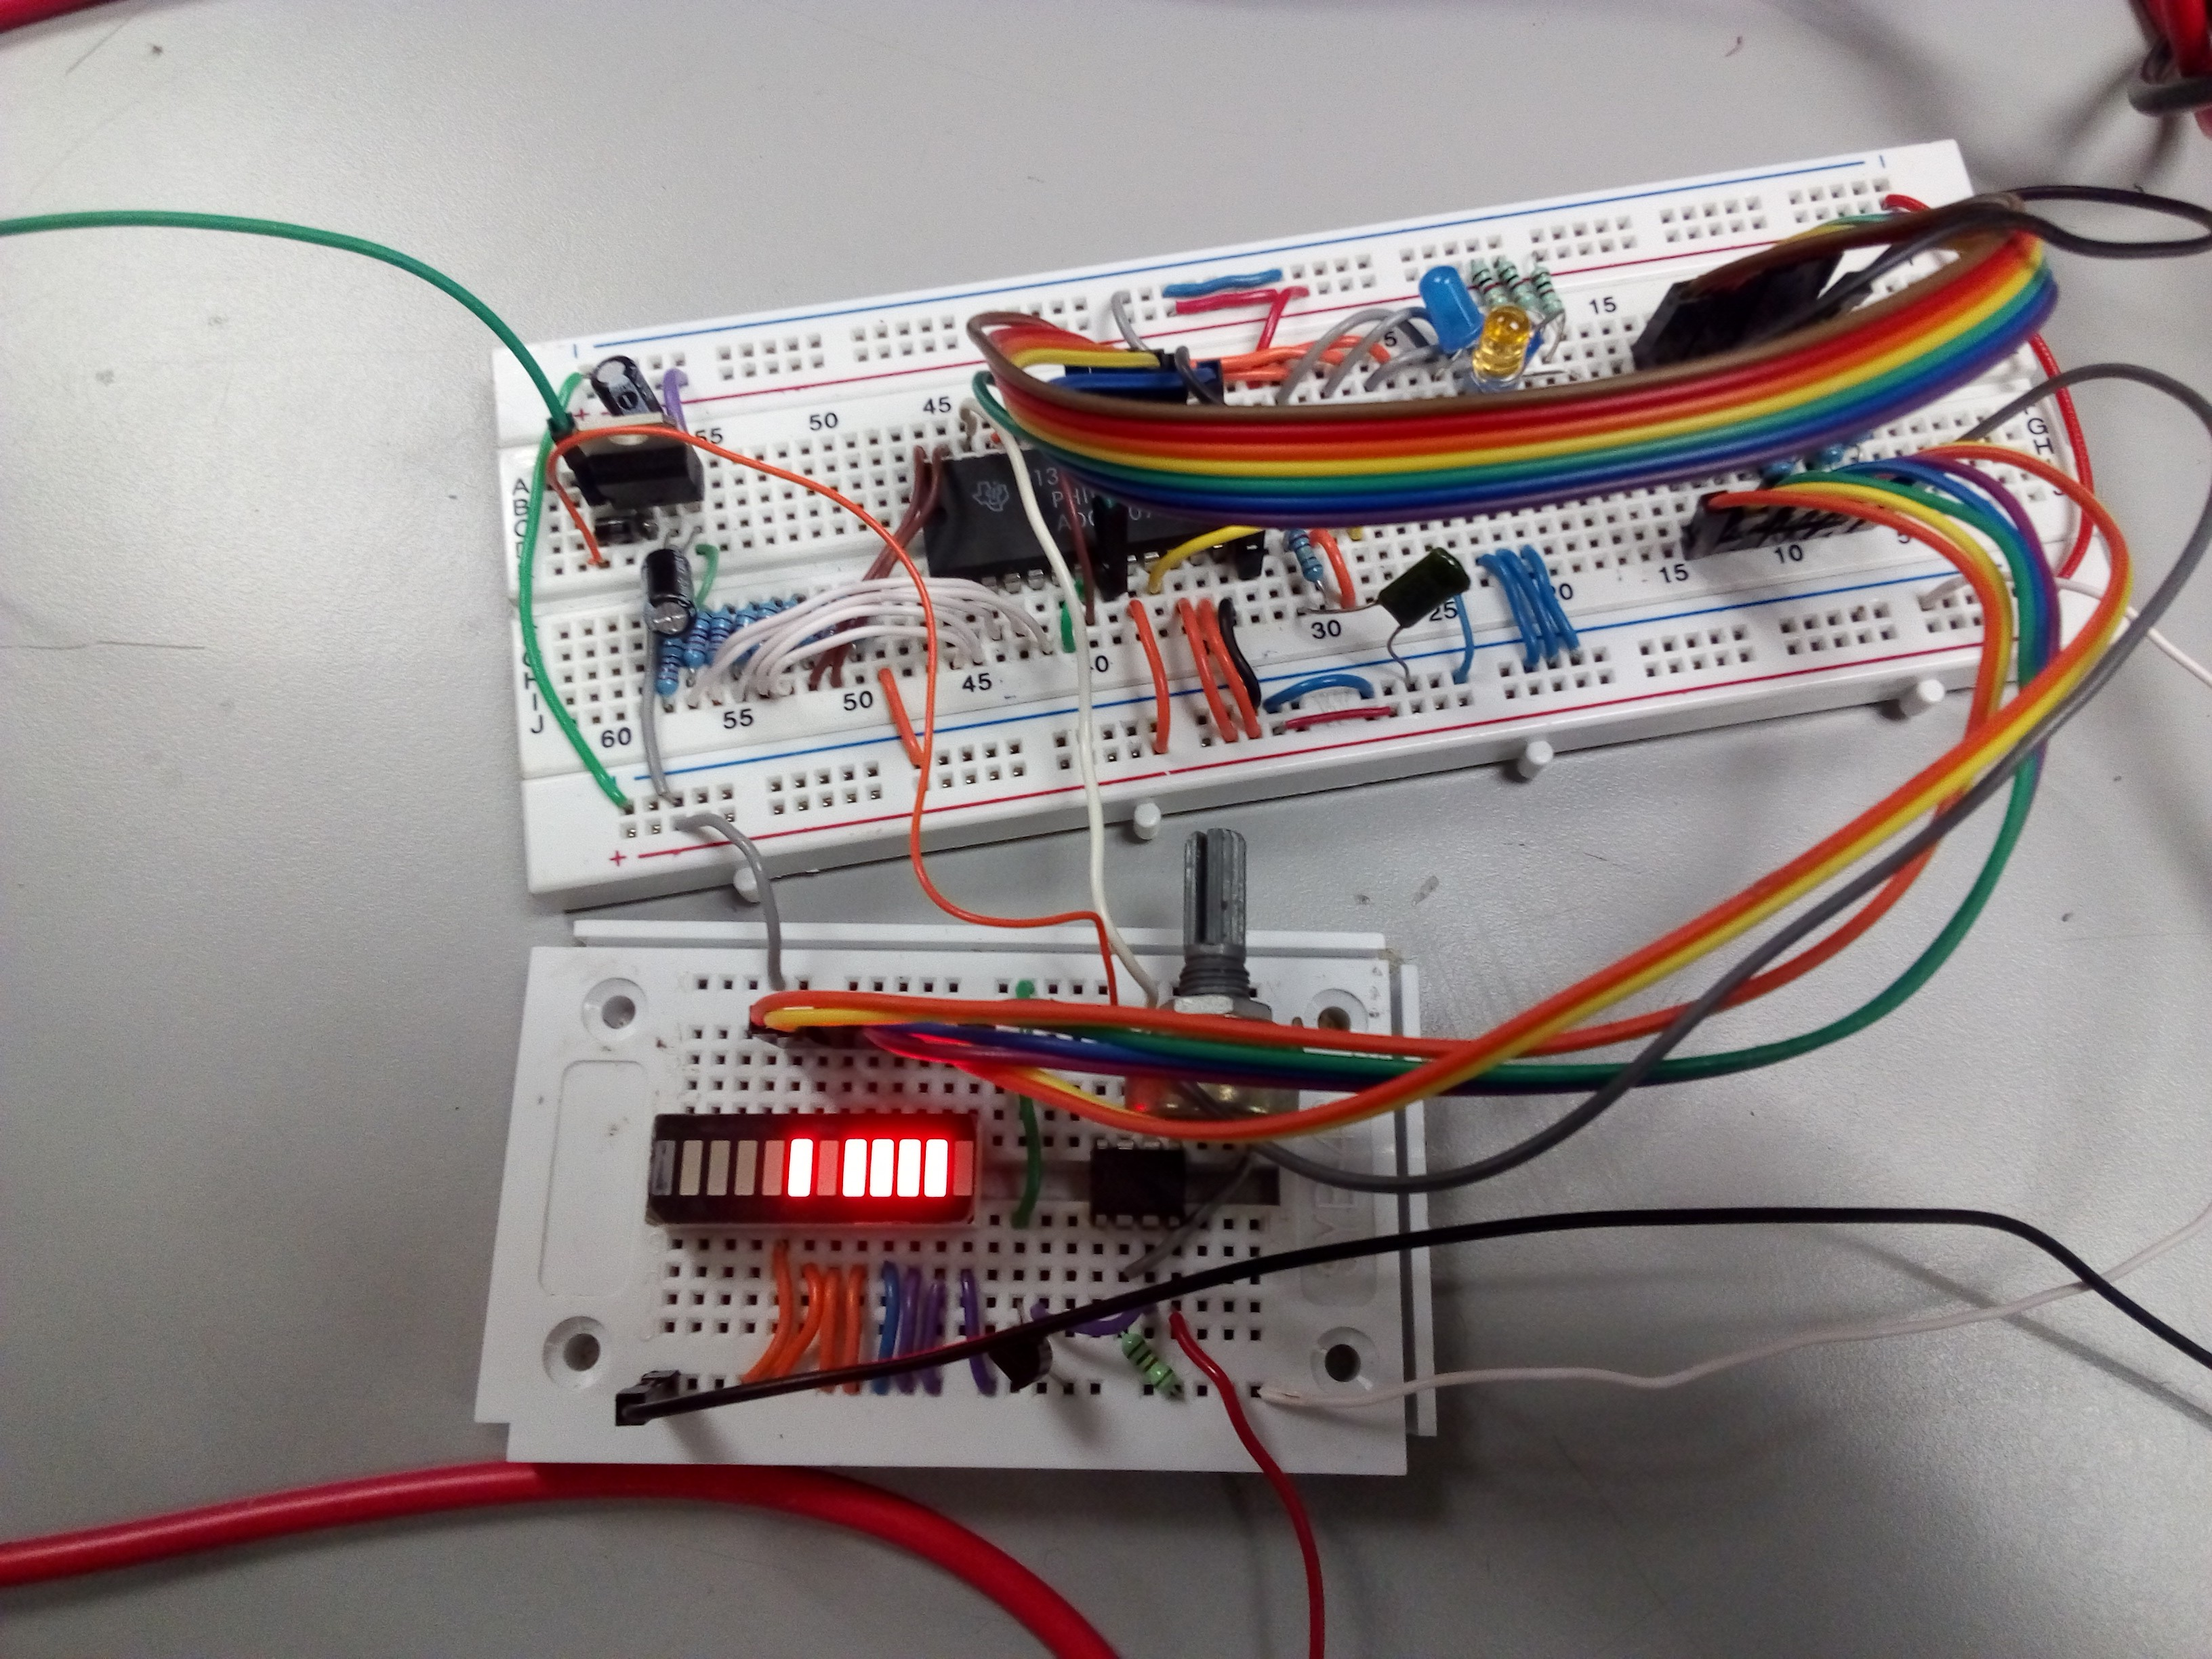
\includegraphics[width=0.68\textwidth]{Practica4/Fotos/temperatura6.jpg}
    \end{figure}
    \newpage
	\subsubsection{Mediciones}
    \textbf{Medición 1}

    \textbf{Voltaje Medido:} 2.2339 V (22.33$^{\circ}$C)
    
    \textbf{Binario en CI:} 01110010
    
    \textbf{Decimal en CI:} 114

    \textbf{Voltaje Teórico:} $114 \times 0.019607 V$ = 2.2352 V (22.35$^{\circ}$C)
    
    \textbf{Decimal Teórico:} = $\frac{2.2339V}{0.019607V}$ = 113
    
    \textbf{Binario Teórico:} 01110001
    
    \textbf{Error de Voltaje:} 2.2352 V - 2.2339 V = 0.0013 V
    
    \textbf{Error de Decimal:} 114 - 113 = 1
    
    \begin{figure}[h!]
                \centering
                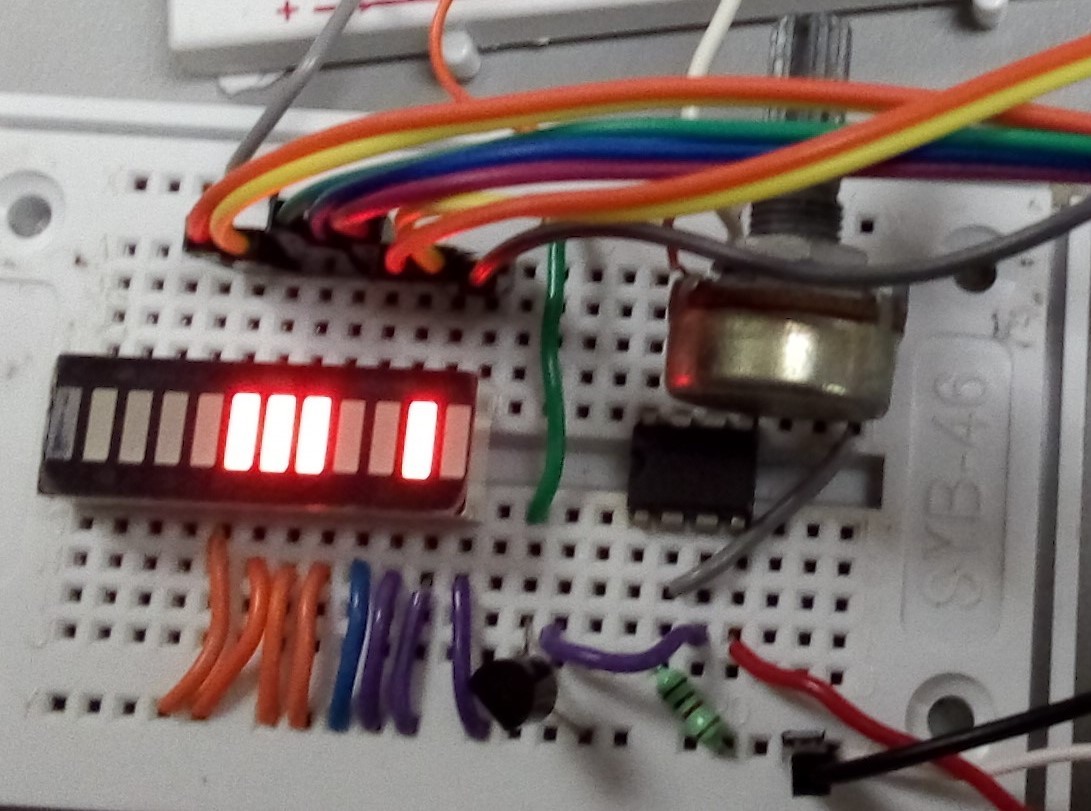
\includegraphics[width=0.7\textwidth]{Practica4/Fotos/med1.jpg}
    \end{figure}
    
    \begin{figure}[h!]
                \centering
                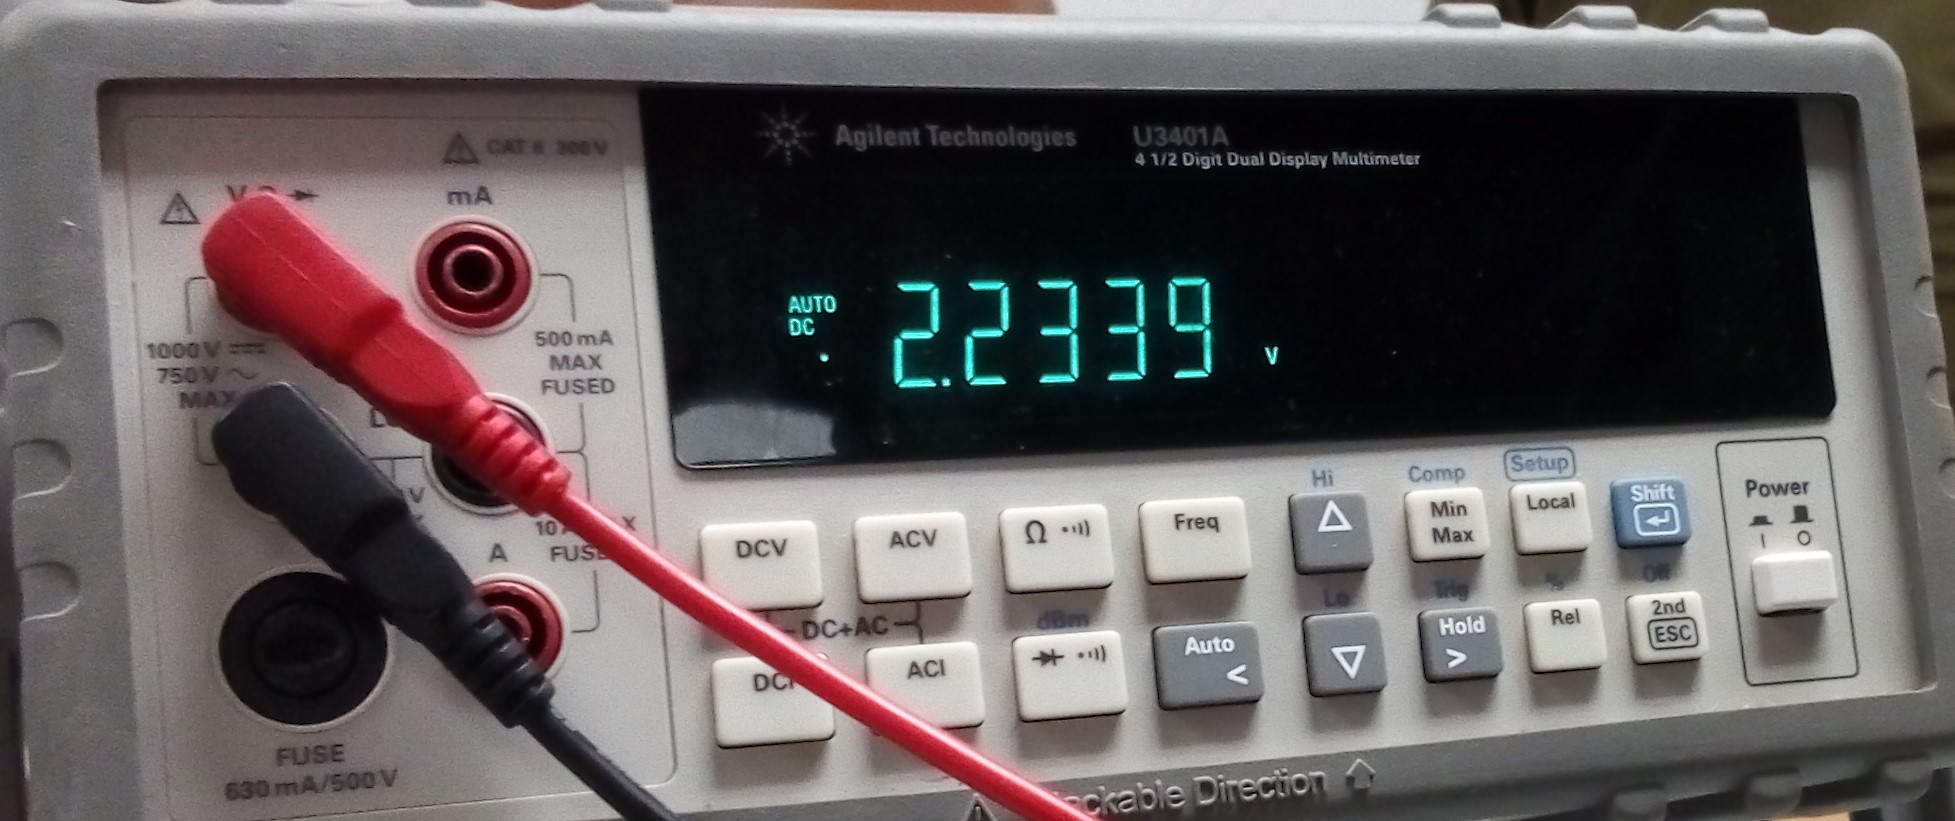
\includegraphics[width=0.7\textwidth]{Practica4/Fotos/voltaje1.jpg}
    \end{figure}
    
    \newpage
    \textbf{Medición 2}

    \textbf{Voltaje Medido:} 2.2469 V (22.46$^{\circ}$C)
    
    \textbf{Binario en CI:} 01110011
    
    \textbf{Decimal en CI:} 115

    \textbf{Voltaje Teórico:} $115 \times 0.019607 V$ = 2.2549 V (22.54$^{\circ}$C)
    
    \textbf{Decimal Teórico:} = $\frac{2.2469V}{0.019607V}$ = 114
    
    \textbf{Binario Teórico:} 01110010
    
    \textbf{Error de Voltaje:} 2.2549 V - 2.2469 V = 0.008 V
    
    \textbf{Error de Decimal:} 115 - 114 = 1
    
    \begin{figure}[h!]
                \centering
                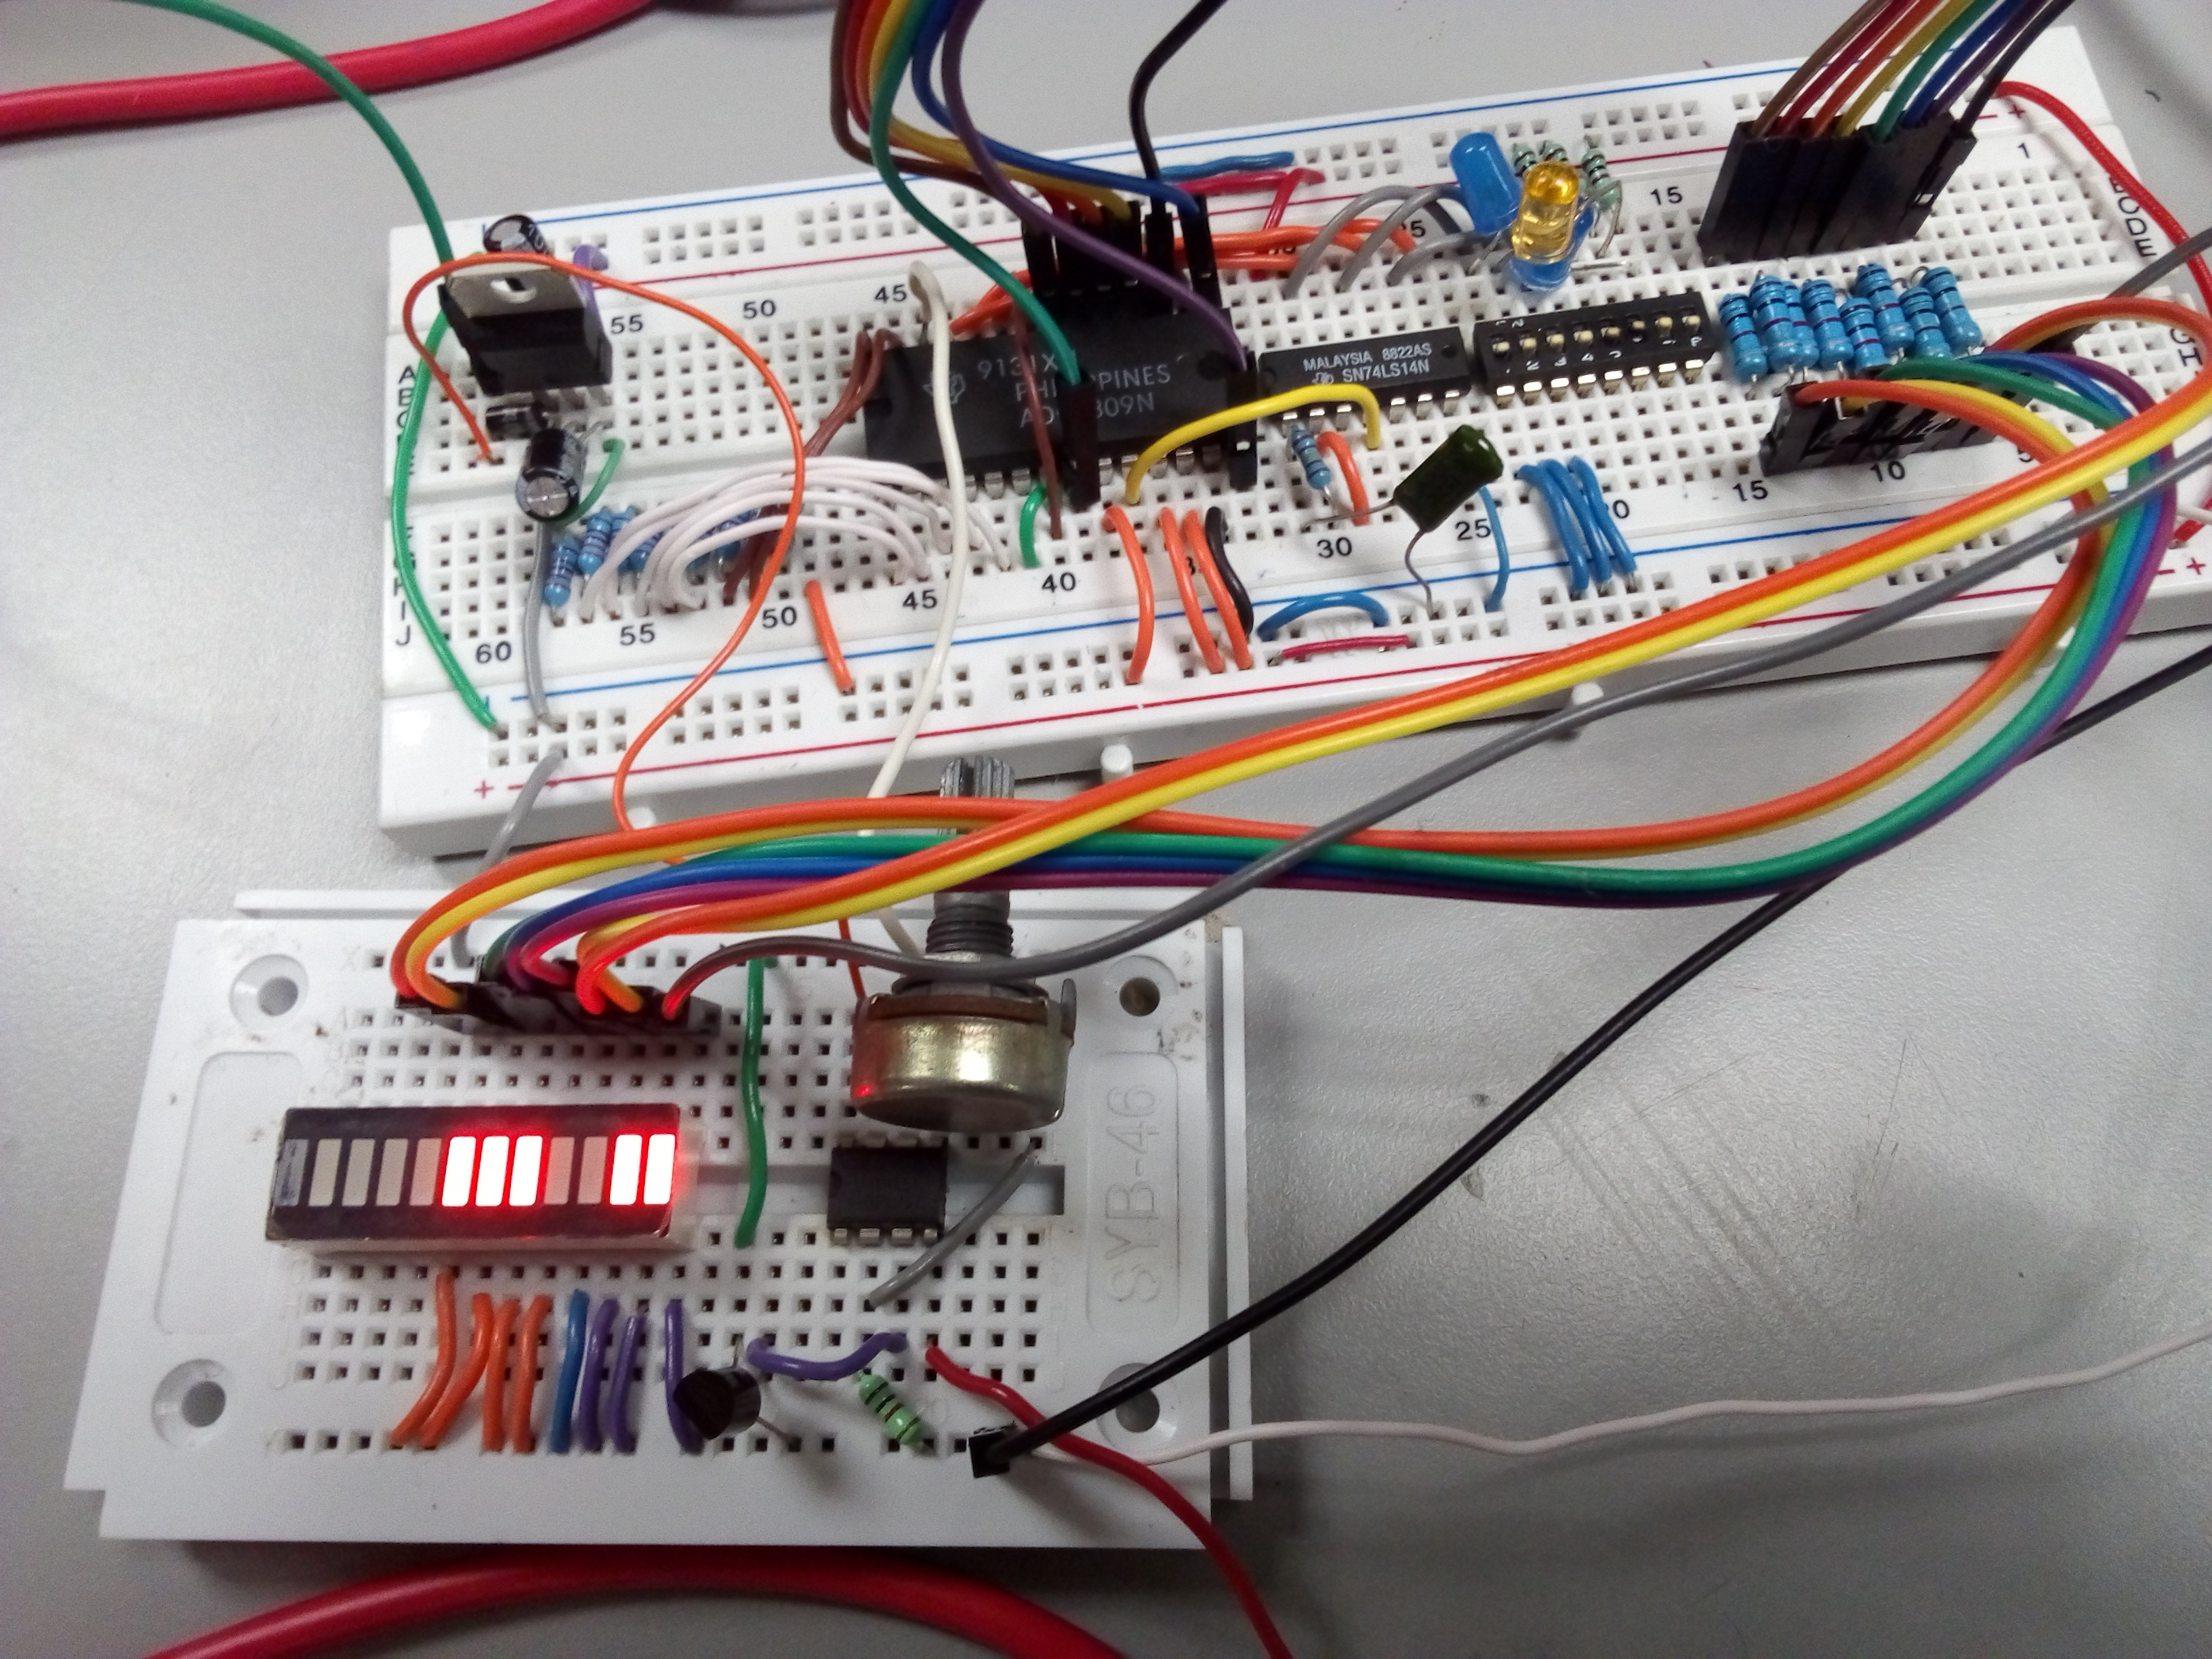
\includegraphics[width=0.7\textwidth]{Practica4/Fotos/med2_2.jpg}
    \end{figure}
    
    \begin{figure}[h!]
                \centering
                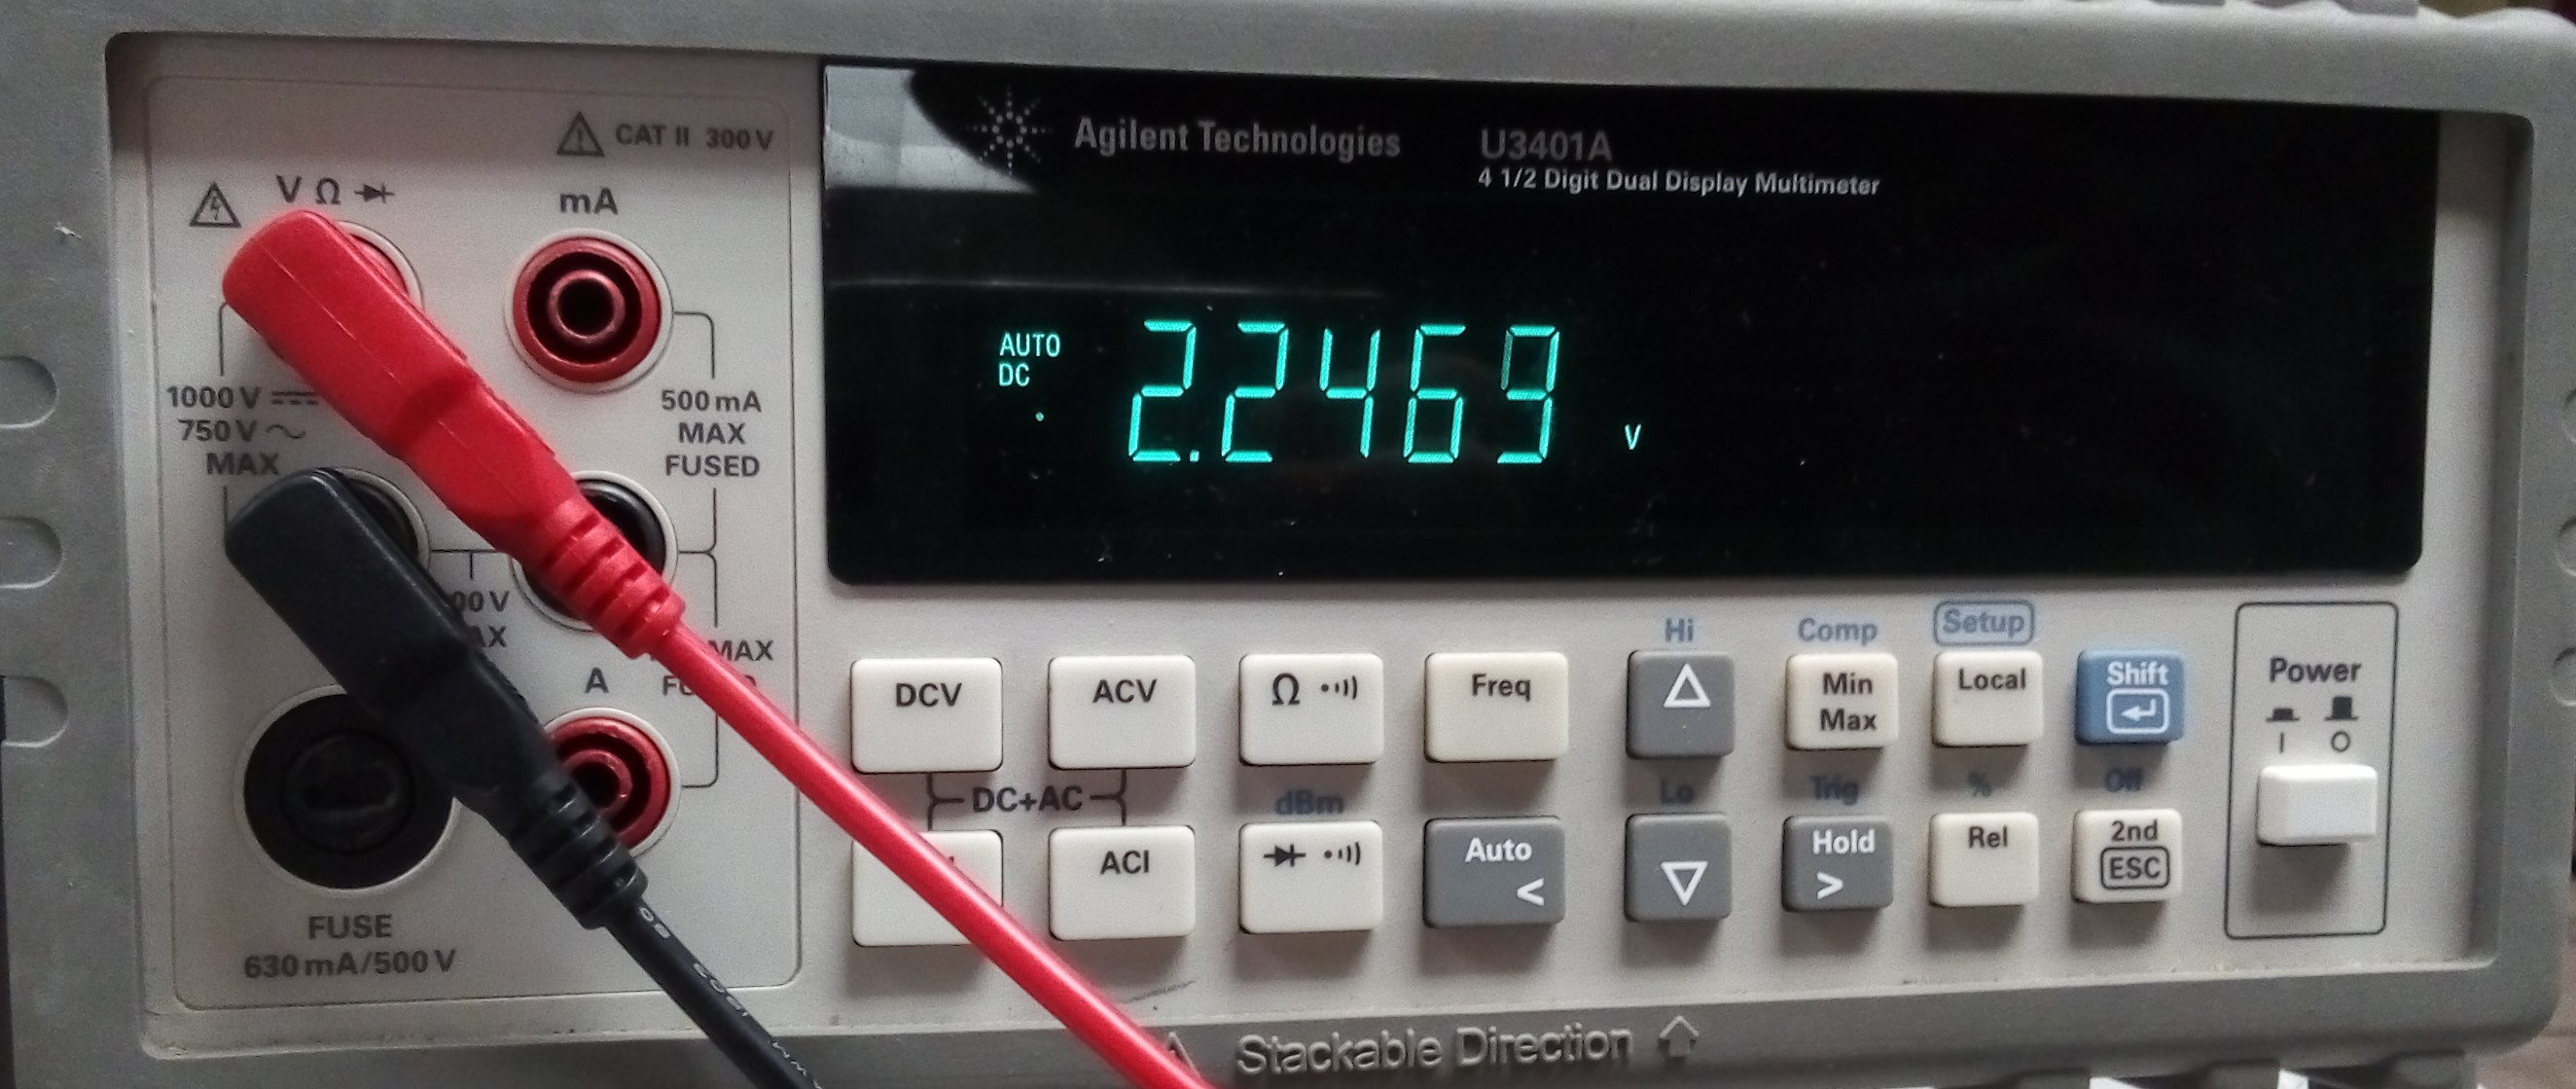
\includegraphics[width=0.7\textwidth]{Practica4/Fotos/voltaje2.jpg}
    \end{figure}


	\newpage
	% /////////////////////////////////////////////////////////////////////
	%							CONCLUSIONES
	% ////////////////////////////////////////////////////////////////////
	\section{Conclusiones}
	    \subsection{Aguilar Herrera Arianna Itzamina}
	    Esta práctica sirvió para medir una variable, la temperatura, utilizando un convertidor Analógico-Digital, obteniendo un voltaje, según la temperatura, asignándole un valor en número binario y decimal. 
	    
	    Para obtener un cálculo más exacto se ocuparon dos temas de instrumentación la resolución y el error. 
	    Nuestra resolución es el valor mínimo que se puede medir, en este caso fue un grado, a partir del cual haciendo los correspondientes cálculos se determinó la temperatura correspondiente a cada voltaje. 
	    Además se llevo a cabo de tal forma que el error fuera de uno, o a lo mucho, dos bits. Vemos que se cumplieron los objetivos.
	    
	    \subsection{Nicolás Sayago Abigail}
	    Al finalizar está práctica pude comprender las características del convertidor Analógico - Digital, siendo este la forma en la que se convierten los valores a una forma más entendible para analizar, en el reporte de la práctica se destaca la importancia puesto que con una señal digital es fácil trabajar la información en una computadora. 
	    
	    Al desarrollar la práctica notamos que existía cierto margen de error y dependiendo de cada circuito era su valor (comparamos con compañeros), es importante notar como afecta esto a los valores que obtenemos.
	    
	    Dichas mediciones se hicieron con la aplicación del sensor de temperatura, que en mi opinión, fue la parte más difícil y todo por no saber conectar bien el circuito.
	    
	    Finalmente, con la aplicación, el convertidor y la medición de error pudimos obtener valores en bits viniendo de una señal analógica.
	    
	    
	    \subsection{Ramos Diaz Enrique}
	    Al medir una variable, las señales que arroja un determinado sensor solamente están conformadas de valores de voltaje, resistencia y corriente eléctrica. En la interpretación de los resultados reales, estos valores carecen de significado y no explican la variable que se esta midiendo.
	    
	    Por esto, con ayuda de un CAD, estas señales analógicas las podemos convertir a valores lógicos, pertenecientes al sistema binario. 
	    
	    Al manejar el sistema binario, podemos darle significado a los valores de voltaje que arroja un sensor, convirtiendo estos a otro sistema numérico, como decimal o hexadecimal.
	    
	    Una vez obtenido este valor un poco más coherente dentro del contexto de la medición, podemos enviarlo por medio de tecnologías como Arduino a algún sistema computacional para desplegar en una pantalla o display esta medida.
	    
	    El ADC0809 maneja un rango de medición de 0 a 255 (8 bits) en sistema binario, y se alimenta con 5V, por lo que su resolución será el voltaje para cada bit, que es valor mínimo a medida (o unidad, en sistema decimal).
	    
	    El error de medición indica que tanto varía el valor medido del valor real.
	    
	    En la implementación práctica del ADC0809, utilizamos un LM35 para medir la temperatura ambiente. Nos dimos cuenta que para cada grado Celsius, el sensor arrojaba 10 mV, pero amplificamos este valor para que ahora por cada grado Celsius, el sensor arrojará 0.1 V. Nuestro rango fue de 0 a 50$^{\circ}$C.
	    
	    Cuando obtenemos el valor en binario de la medición de este sensor, ya solo queda establecer una escala entre el binario obtenido en decimal y los grados Celsius que le corresponden a cada valor del rango.
	    

		\newpage
	%/////////////////////////////////////////////////////////////////
	%							ANEXOS
	%/////////////////////////////////////////////////////////////////
	
	\section{Anexos}
	    \subsection{LM741}
	        \begin{figure}[h!]
                \centering
                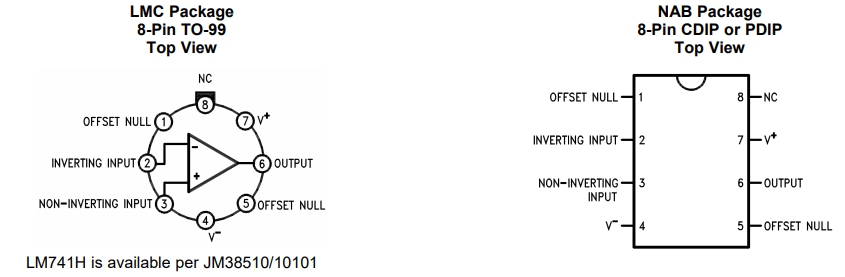
\includegraphics[width=\textwidth]{Practica4/Images/lm741.PNG}
            \end{figure} 
	        El amplificador operacional LM741 debe estar alimentados por una fuente de +12 V y -12 V en serie. Deben ir dos capacitores de $10\mu F$, uno por cada entrada de voltaje. [Consultar hoja de especificaciones del LM741].
	        
	        \begin{figure}[h!]
                \centering
                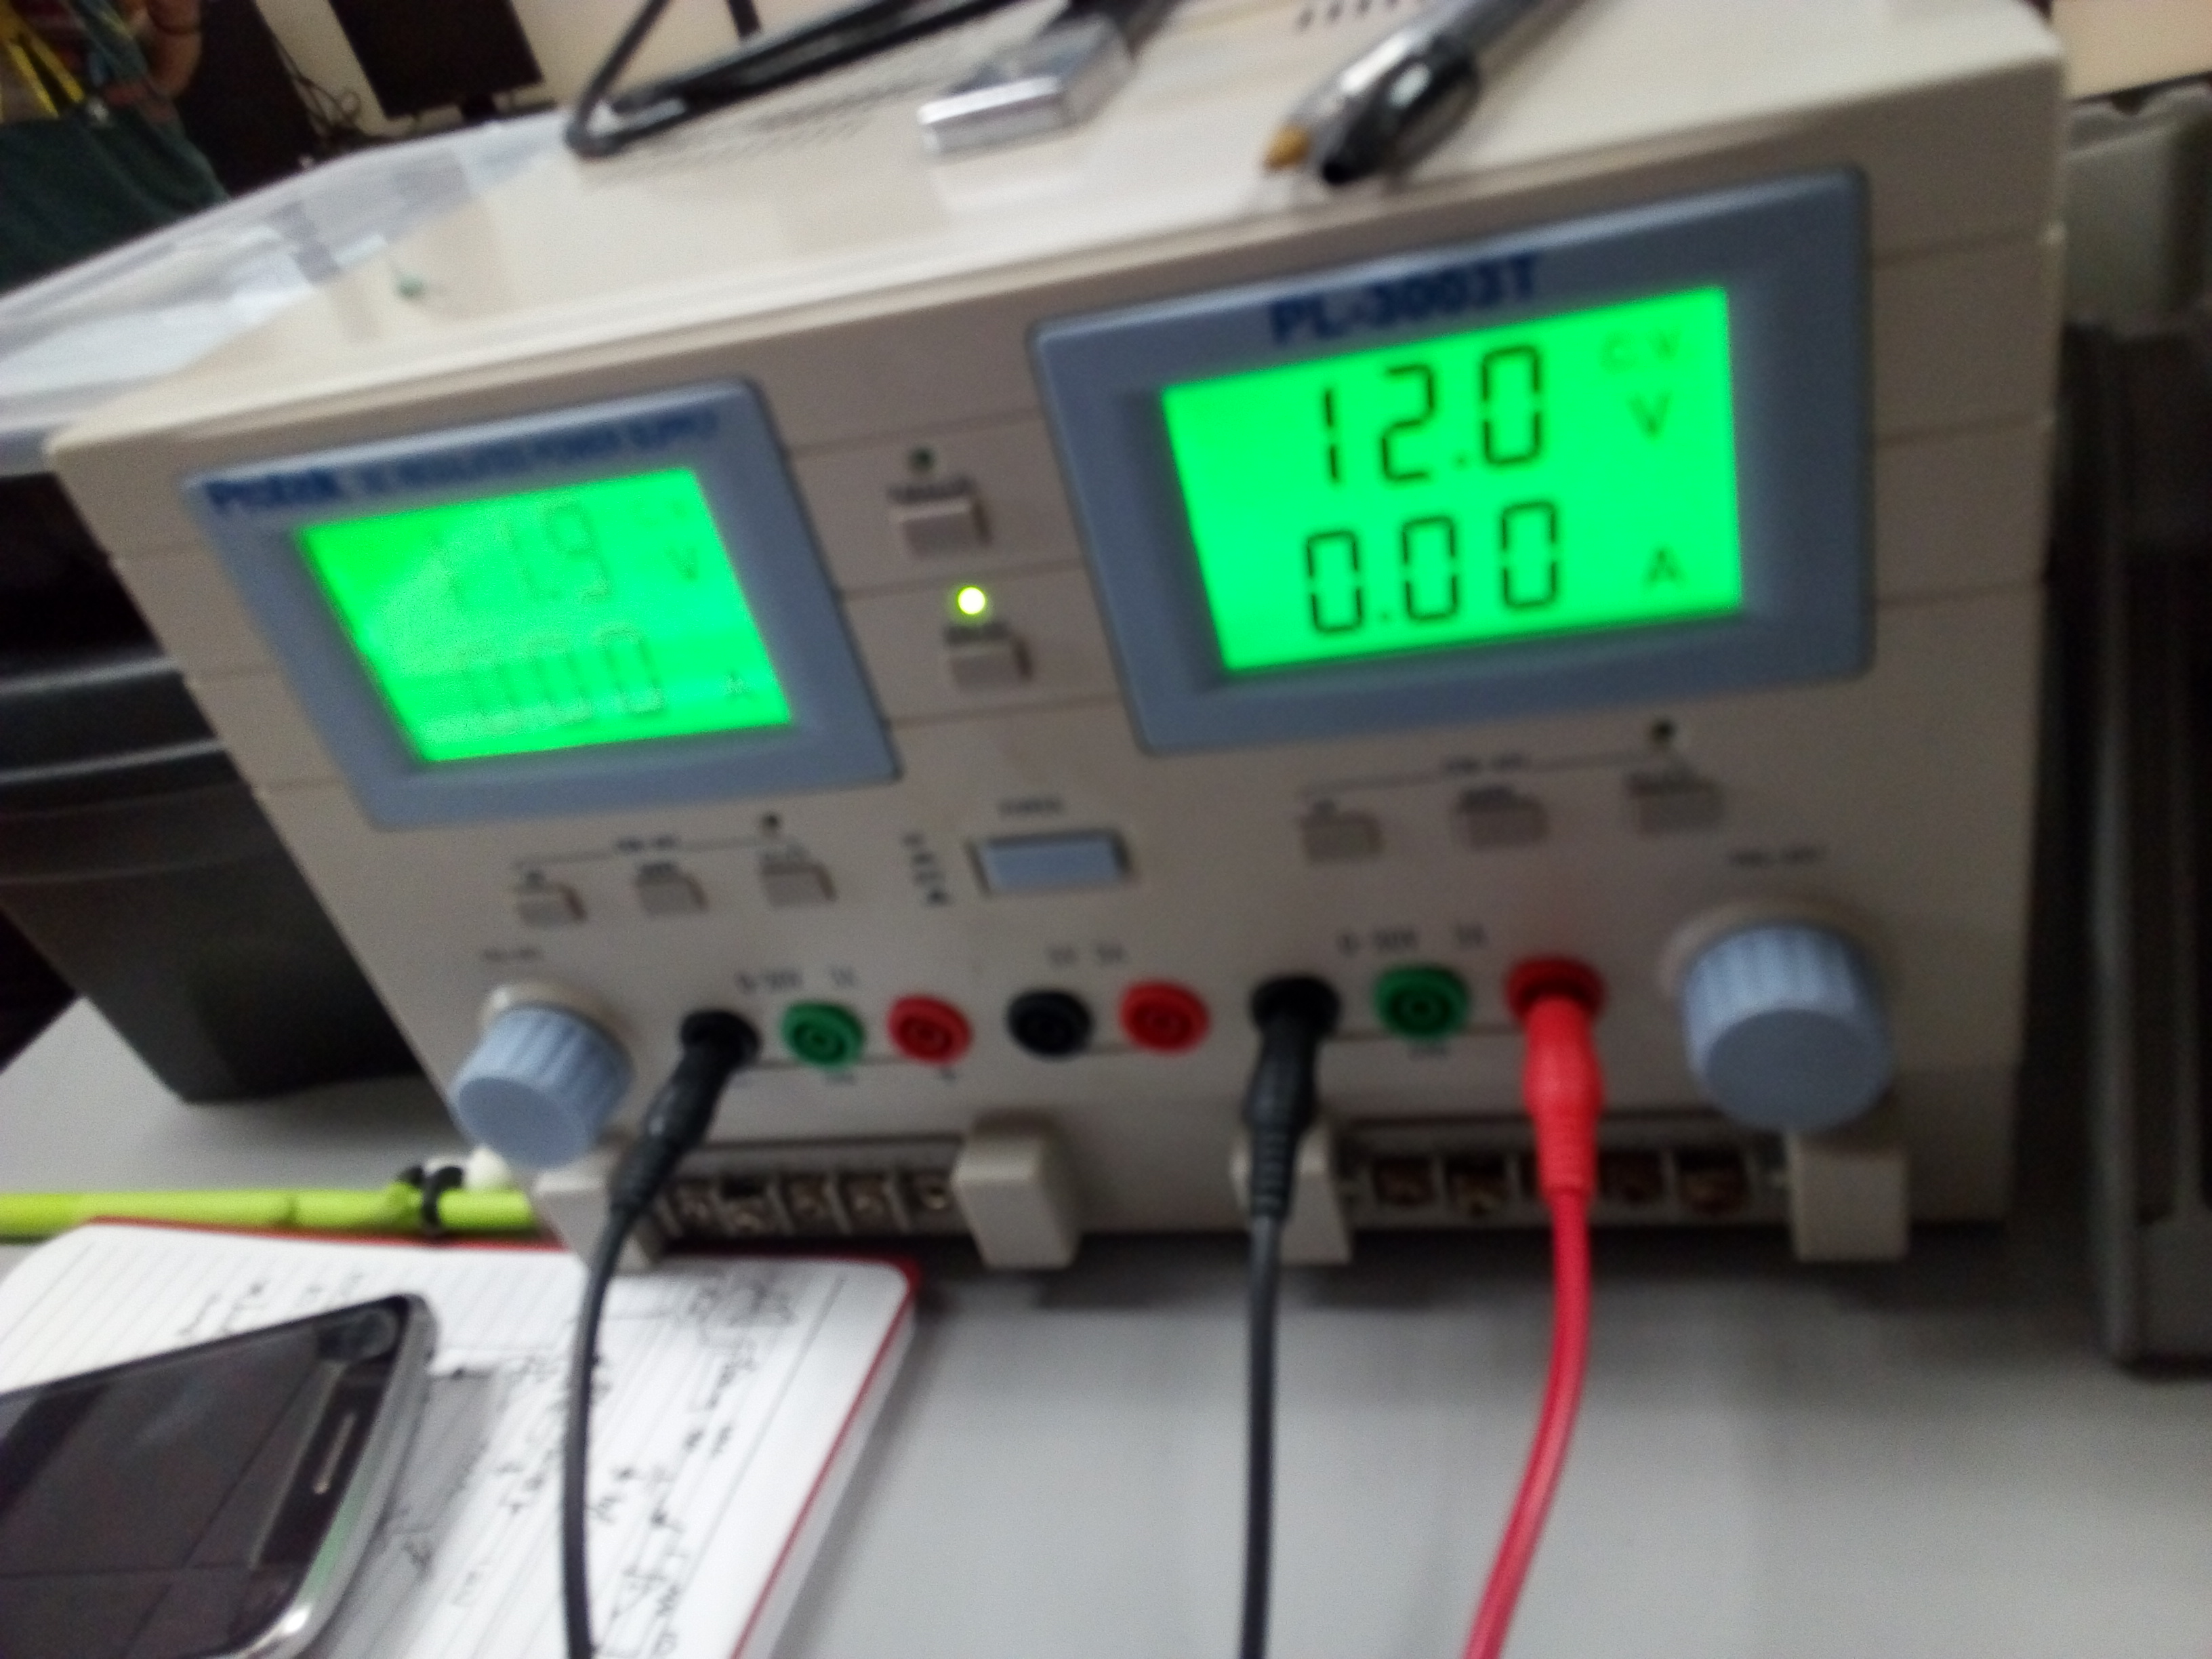
\includegraphics[width=0.7\textwidth]{Sismografo/Images/fuente.jpg}
            \end{figure} 
            
        \newpage
        \subsection{LM7805}
        En el regulador de voltaje LM7805, deben ir cableados dos capacitores de $0.1\mu F$, como se muestra en el siguiente esquema: [Consultar hoja de especificaciones del LM7805].
        
        \begin{figure}[h!]
                \centering
                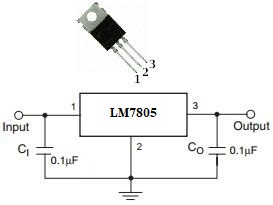
\includegraphics[width=0.55\textwidth]{Practica4/Images/7805.jpg}
            \end{figure}
        
        \subsection{ADC0809}
        El ADC0809 es un conversor de 8 bits (la señal análoga se convierte en una palabra de 8 bits), que tiene la posibilidad de leer 8 señales analógicas (8 canales). Posee 28 pines de los cuales 8 corresponden a los ocho canales de entradas analógicos; éste solo puede leer un canal a la vez y dispone por lo tanto de un selector (multiplexor) de 3 líneas digitales, que permite escoger la señal de entrada a convertir, mediante el código binario.
        
        \begin{figure}[h!]
                \centering
                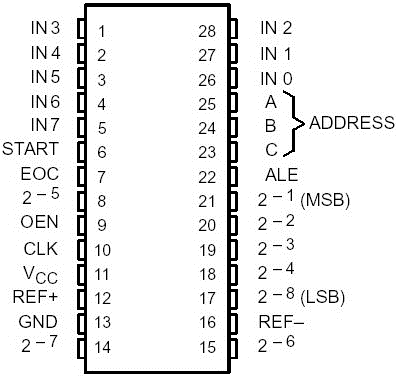
\includegraphics[scale=0.8]{Practica4/Images/adc.png}
            \end{figure}
            \newpage
        \subsection{LM35 Sensor de temperatura integrado}
        El LM35 es un dispositivo de tres terminales que produce un voltaje de salida 10mV/$^{\circ}$C, de modo que el voltaje nominal de salida es 250mV a 25$^{\circ}$C y 1V a 100$^{\circ}$C. Este sensor puede medir temperaturas debajo de 0$^{\circ}$C usando una resistencia de pull-down desde el terminal de salida a una tensión debajo de cero. La precisión del LM35 es de $\pm$1º C desde -55ºC a +150$^{\circ}$C. 
        \begin{center}
            
        
        \subfigure{ 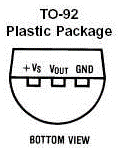
\includegraphics[scale=1.3]{Practica4/Images/lm35_1.png}}
        \subfigure{
        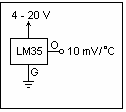
\includegraphics[scale=1.3]{Practica4/Images/lm35_2.png}}
        \end{center}
        
        \subsection{Inversor SN74LS14N}
        \begin{figure}[h!]
                \centering
                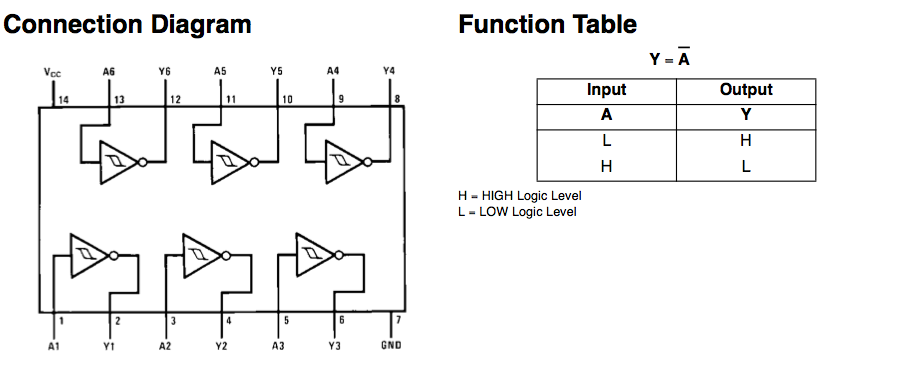
\includegraphics[width=\textwidth]{Practica4/Images/sn7414n.png}
        \end{figure}
            
            
            %/////////////////////////////////////////////////////////////////
    	%          CALCULOS PROCEDIMIENTO EXPERIMENTAL 4
    	%/////////////////////////////////////////////////////////////////
    	\newpage
		\subsection{Cálculos PE 3 - Acondicionamiento de la entradas del sensor de temperatura}
		
		\item Definimos la ganancia de voltaje $A_{CL}$ en la etapa de medición de temperatura, donde el voltaje de entrada es de $V_{i}=500 mV (50^{\circ}C)$ y el voltaje de salida deseado sera de $V_{o}=5 V$
        		
        Aplicando las fórmulas del Amplificador No Inversor tenemos:

        				$$ A_{CL} = \frac{V_{o}}{V{i}} = \frac{5 V}{0.5 V} = 10 $$
        				
        				
        	\item Ahora, utilizamos otra formula que igualaremos con la ecuación anterior:
        	
        	$$ A_{CL} =
        				10 = 1 + \frac{R_{1}}{R_{2}} $$
        				
            \item Comenzamos a operar en ella. Pasamos el uno restando al otro lado de la igualdad:
            
            $$ 9 = \frac{R_{1}}{R_{2}} $$
        	
        	\item Como vemos, obtuvimos una única ecuación pero con 2 incógnitas. Matemáticamente es imposible solucionar esto. Para evitar quedarnos estancados proponemos un valor para cualquiera de las resistencias. En esta caso elegimos $R_{2} = 1K\Omega$
        	\\
        	$$ 9 = \frac{R_{1}}{1K\Omega} $$
            
            \item Pasando $1K\Omega$ multiplicando, obtenemos $R_{1}$
            \\
            $$ R_{1} = (9)(1K\Omega) = 9K\Omega $$
            
            \item Los valores de las resistencias son: $R_{1} = 9K\Omega$ y $R_{2} = 1K\Omega$
		

    %/////////////////////////////////////////////////////////////////
	%                           REFERENCIAS
	%/////////////////////////////////////////////////////////////////

	\nocite{ref1}
	\bibliography{ref4}
        

	\end{document}
